% !TeX root = ../main.tex

\chapter{Results}
\section{Taiwan Mandarin and Taiwan Southern Min tones under coarticulation}

\subsection{Tone contours}

Tone contours of Taiwan Mandarin and Taiwan Southern Min tones in carryover and anticipatory positions are shown in Appendix \ref{Appendix:ToneContours}.

\subsection{Directionalities and magnitudes of coarticulatory effects in the two languages}

Tonal coarticulation of Taiwan Mandarin and Taiwan Southern Min in carry-over and anticipatory positions respectively are shown in figures \ref{Figure:LMMCarryover} and \ref{Figure:LMMAnticipatory}. Rather similar distributions of coarticulatory effects were found for both languages. For both languages, in both positions, the ambient tones were shown to exert positive impacts on the target tones, that is, a high ambient tone raised, and a low ambient tone lowered the target tone. In terms of magnitudes, for both positions, no significant difference was found between the two languages. Meaning the two languages showed a similar degree of carry-over and anticipatory effects. Within-language comparisons also revealed essentially no difference between the two kinds of effects in both Taiwan Mandarin and Taiwan Southern Min.

\begin{figure}[hbt!]
\centering
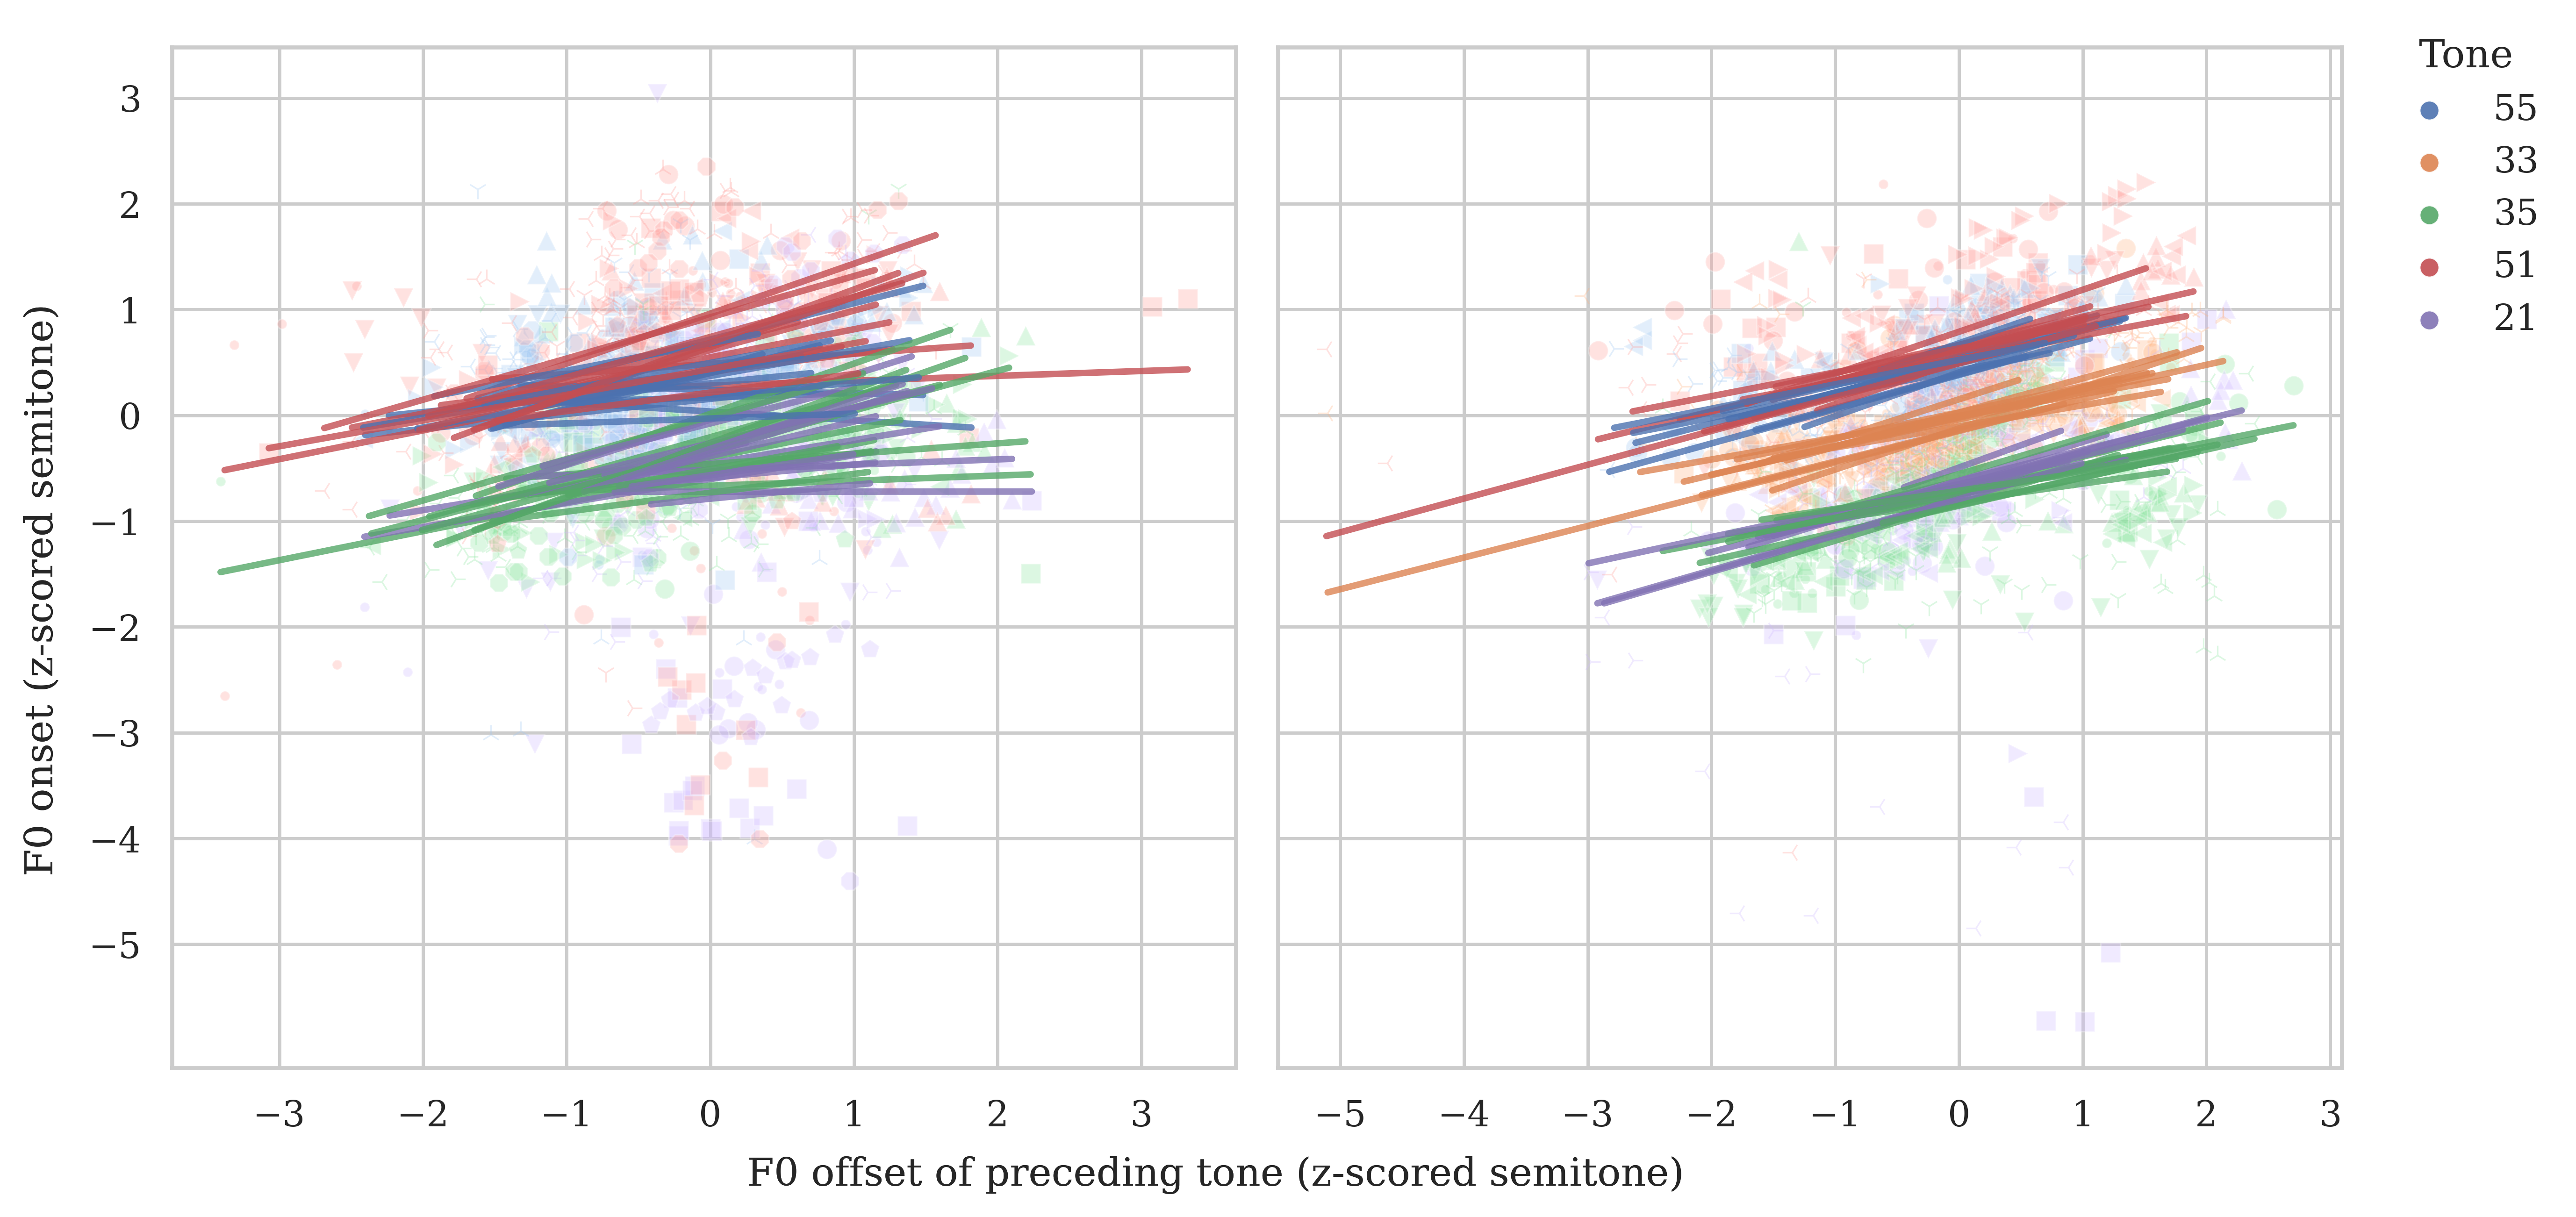
\includegraphics[width=\textwidth, trim={0 .5cm 0 0}]{figures/E1/Carryover_lang_seperated.png}
\caption{Fitted LMM model of tone onsets and offsets in carry-over positions (left: Taiwan Mandarin; right: Taiwan Southern Min).}
\label{Figure:LMMCarryover}
\end{figure}

\begin{figure}[hbt!]
\centering
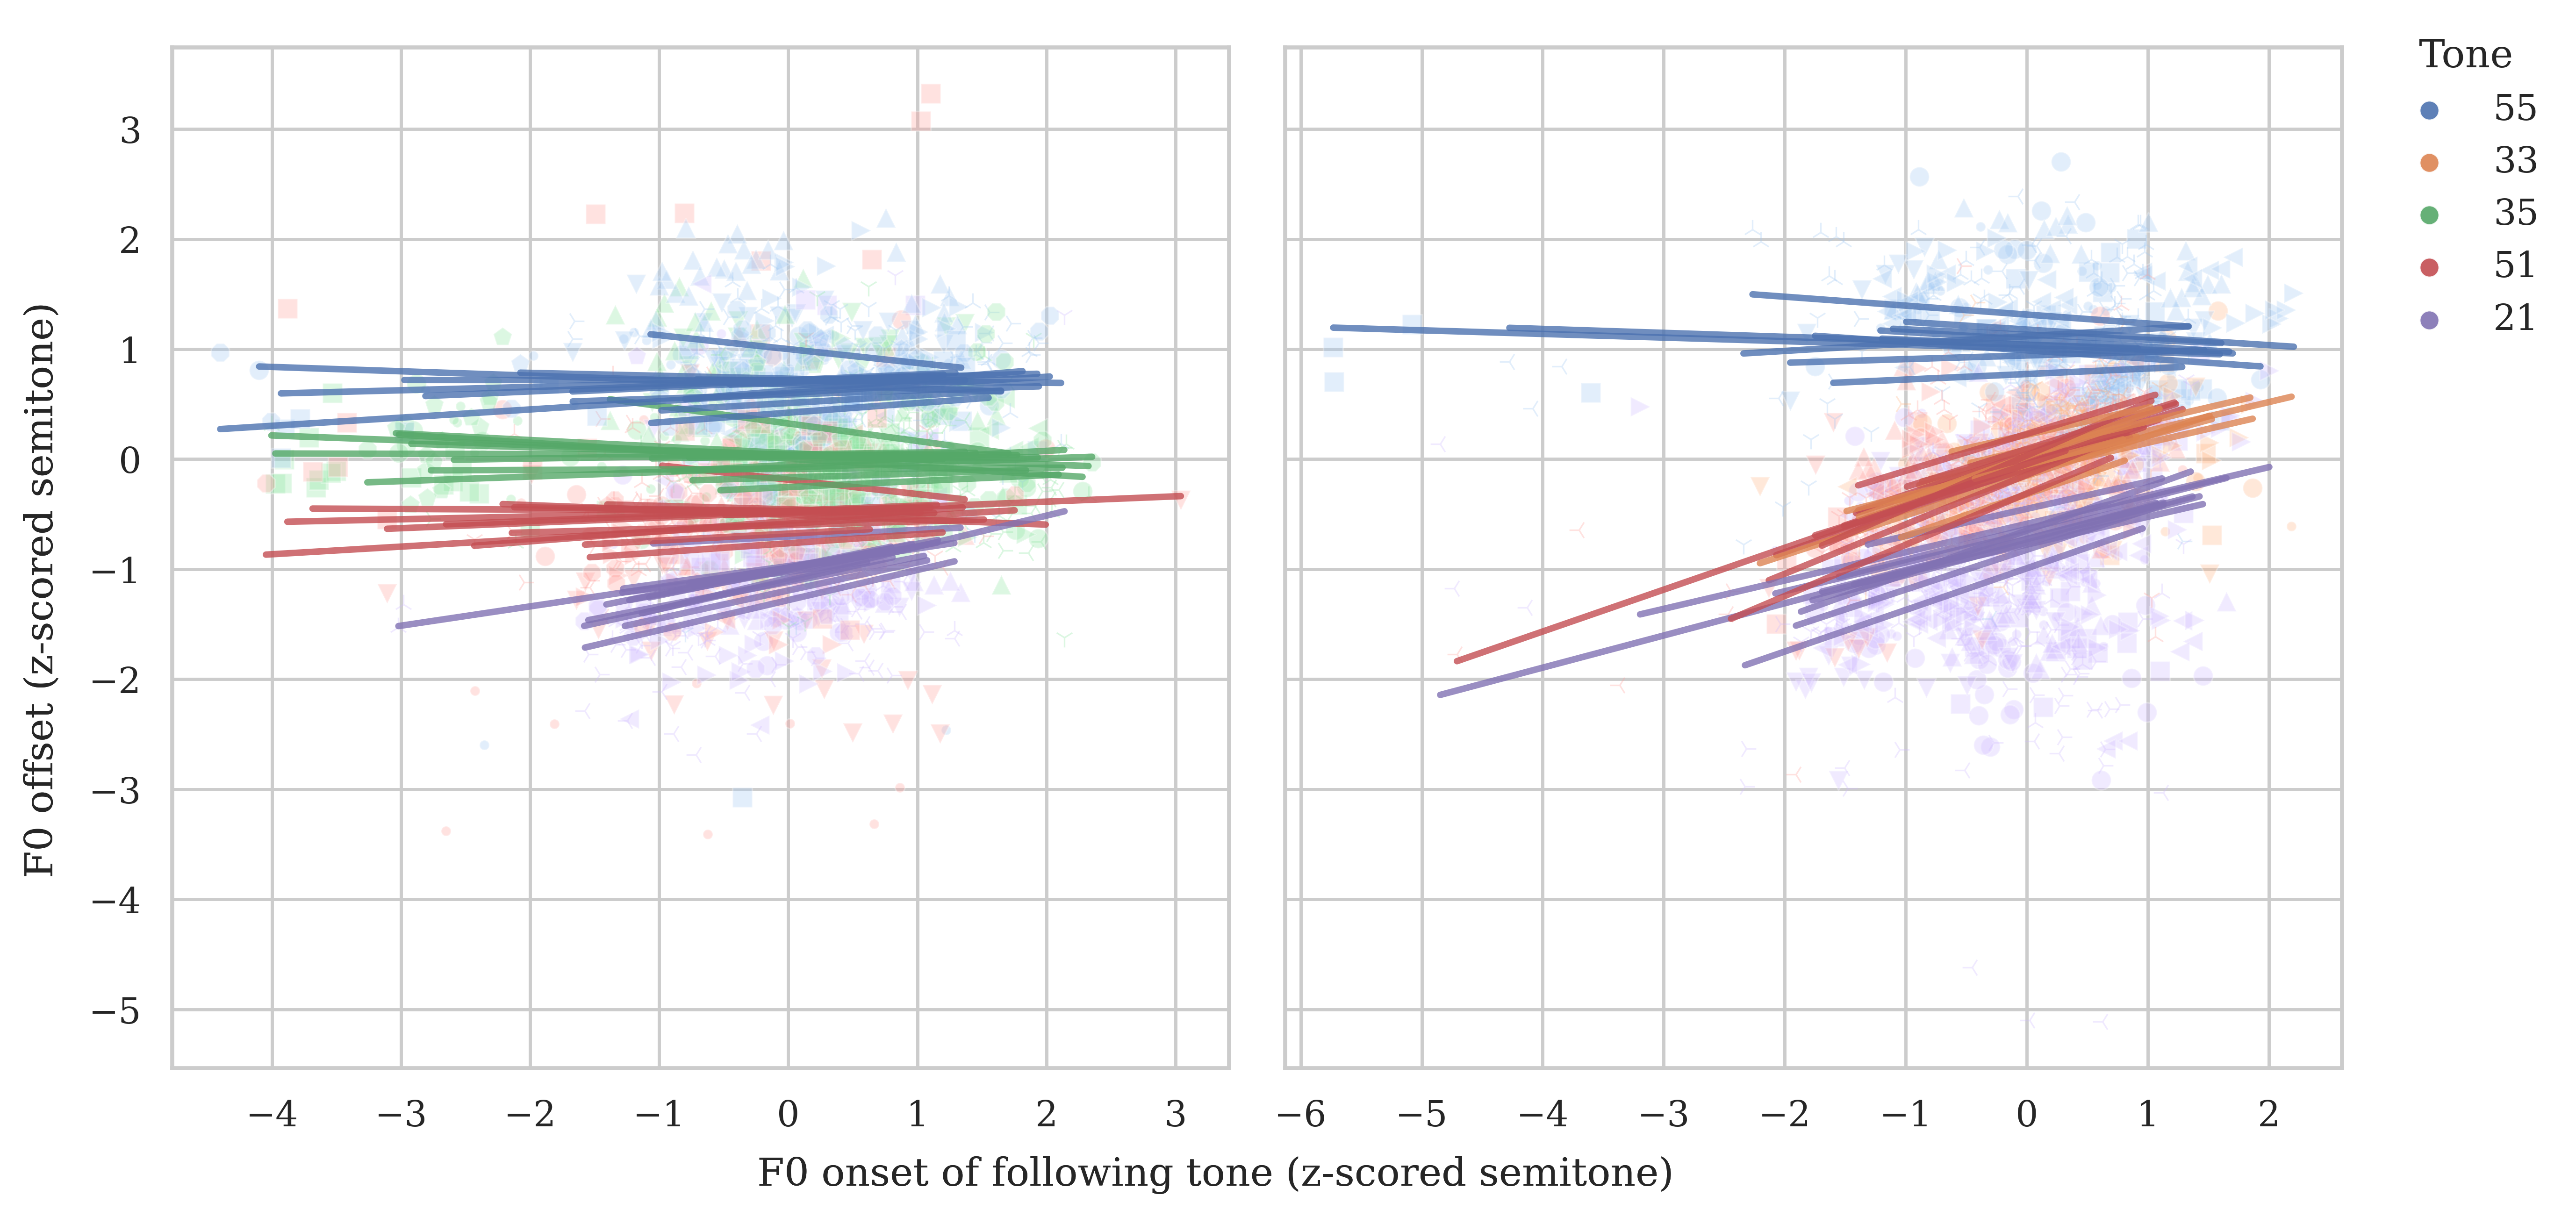
\includegraphics[width=\textwidth, trim={0 .5cm 0 0}]{figures/E1/Anticipatory_lang_seperated.png}
\caption{Fitted LMM model of tone onsets and offsets in anticipatory positions (left: Taiwan Mandarin; right: Taiwan Southern Min).}
\label{Figure:LMMAnticipatory}
\end{figure}

%\begin{figure}[hbt!]
%\centering
%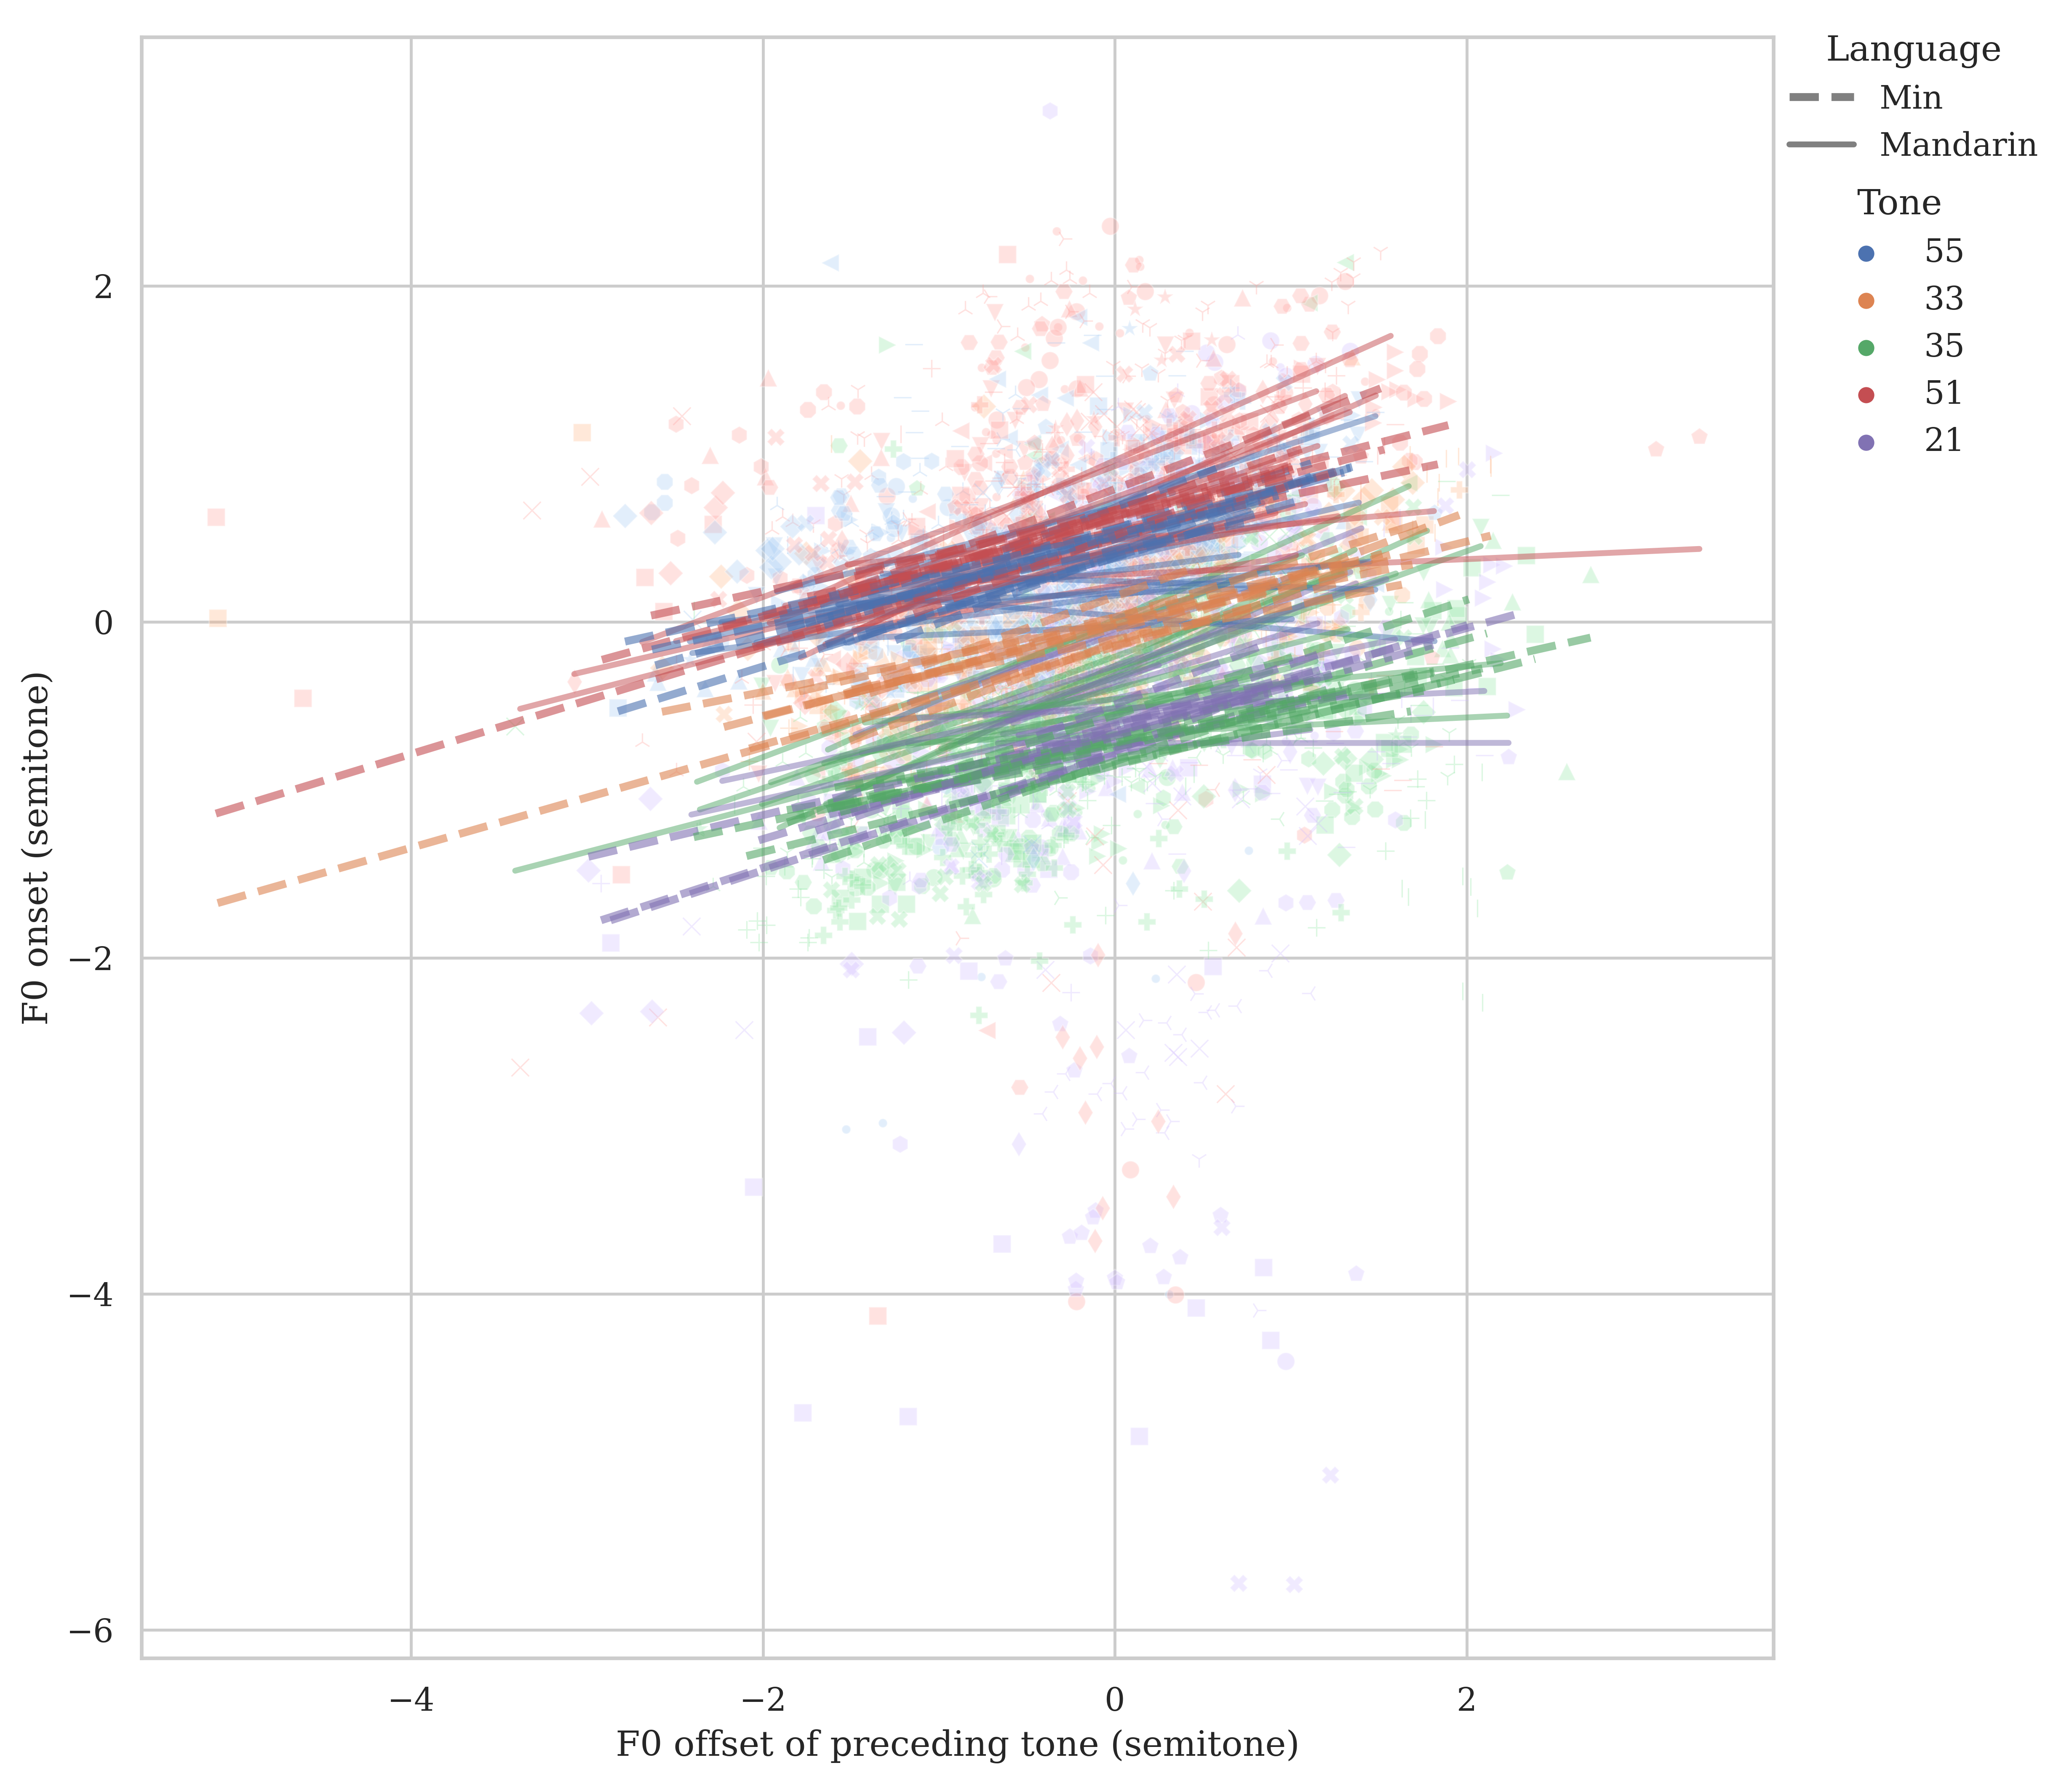
\includegraphics[scale=.45, trim={0 .5cm 0 0}]{figures/E1/Carryover.png}
%\caption{Fitted LMM model of tone onsets and offsets in carry-over positions.}
%\label{Figure:LMMCarryover}
%\end{figure}
%
%\begin{figure}[hbt!]
%\centering
%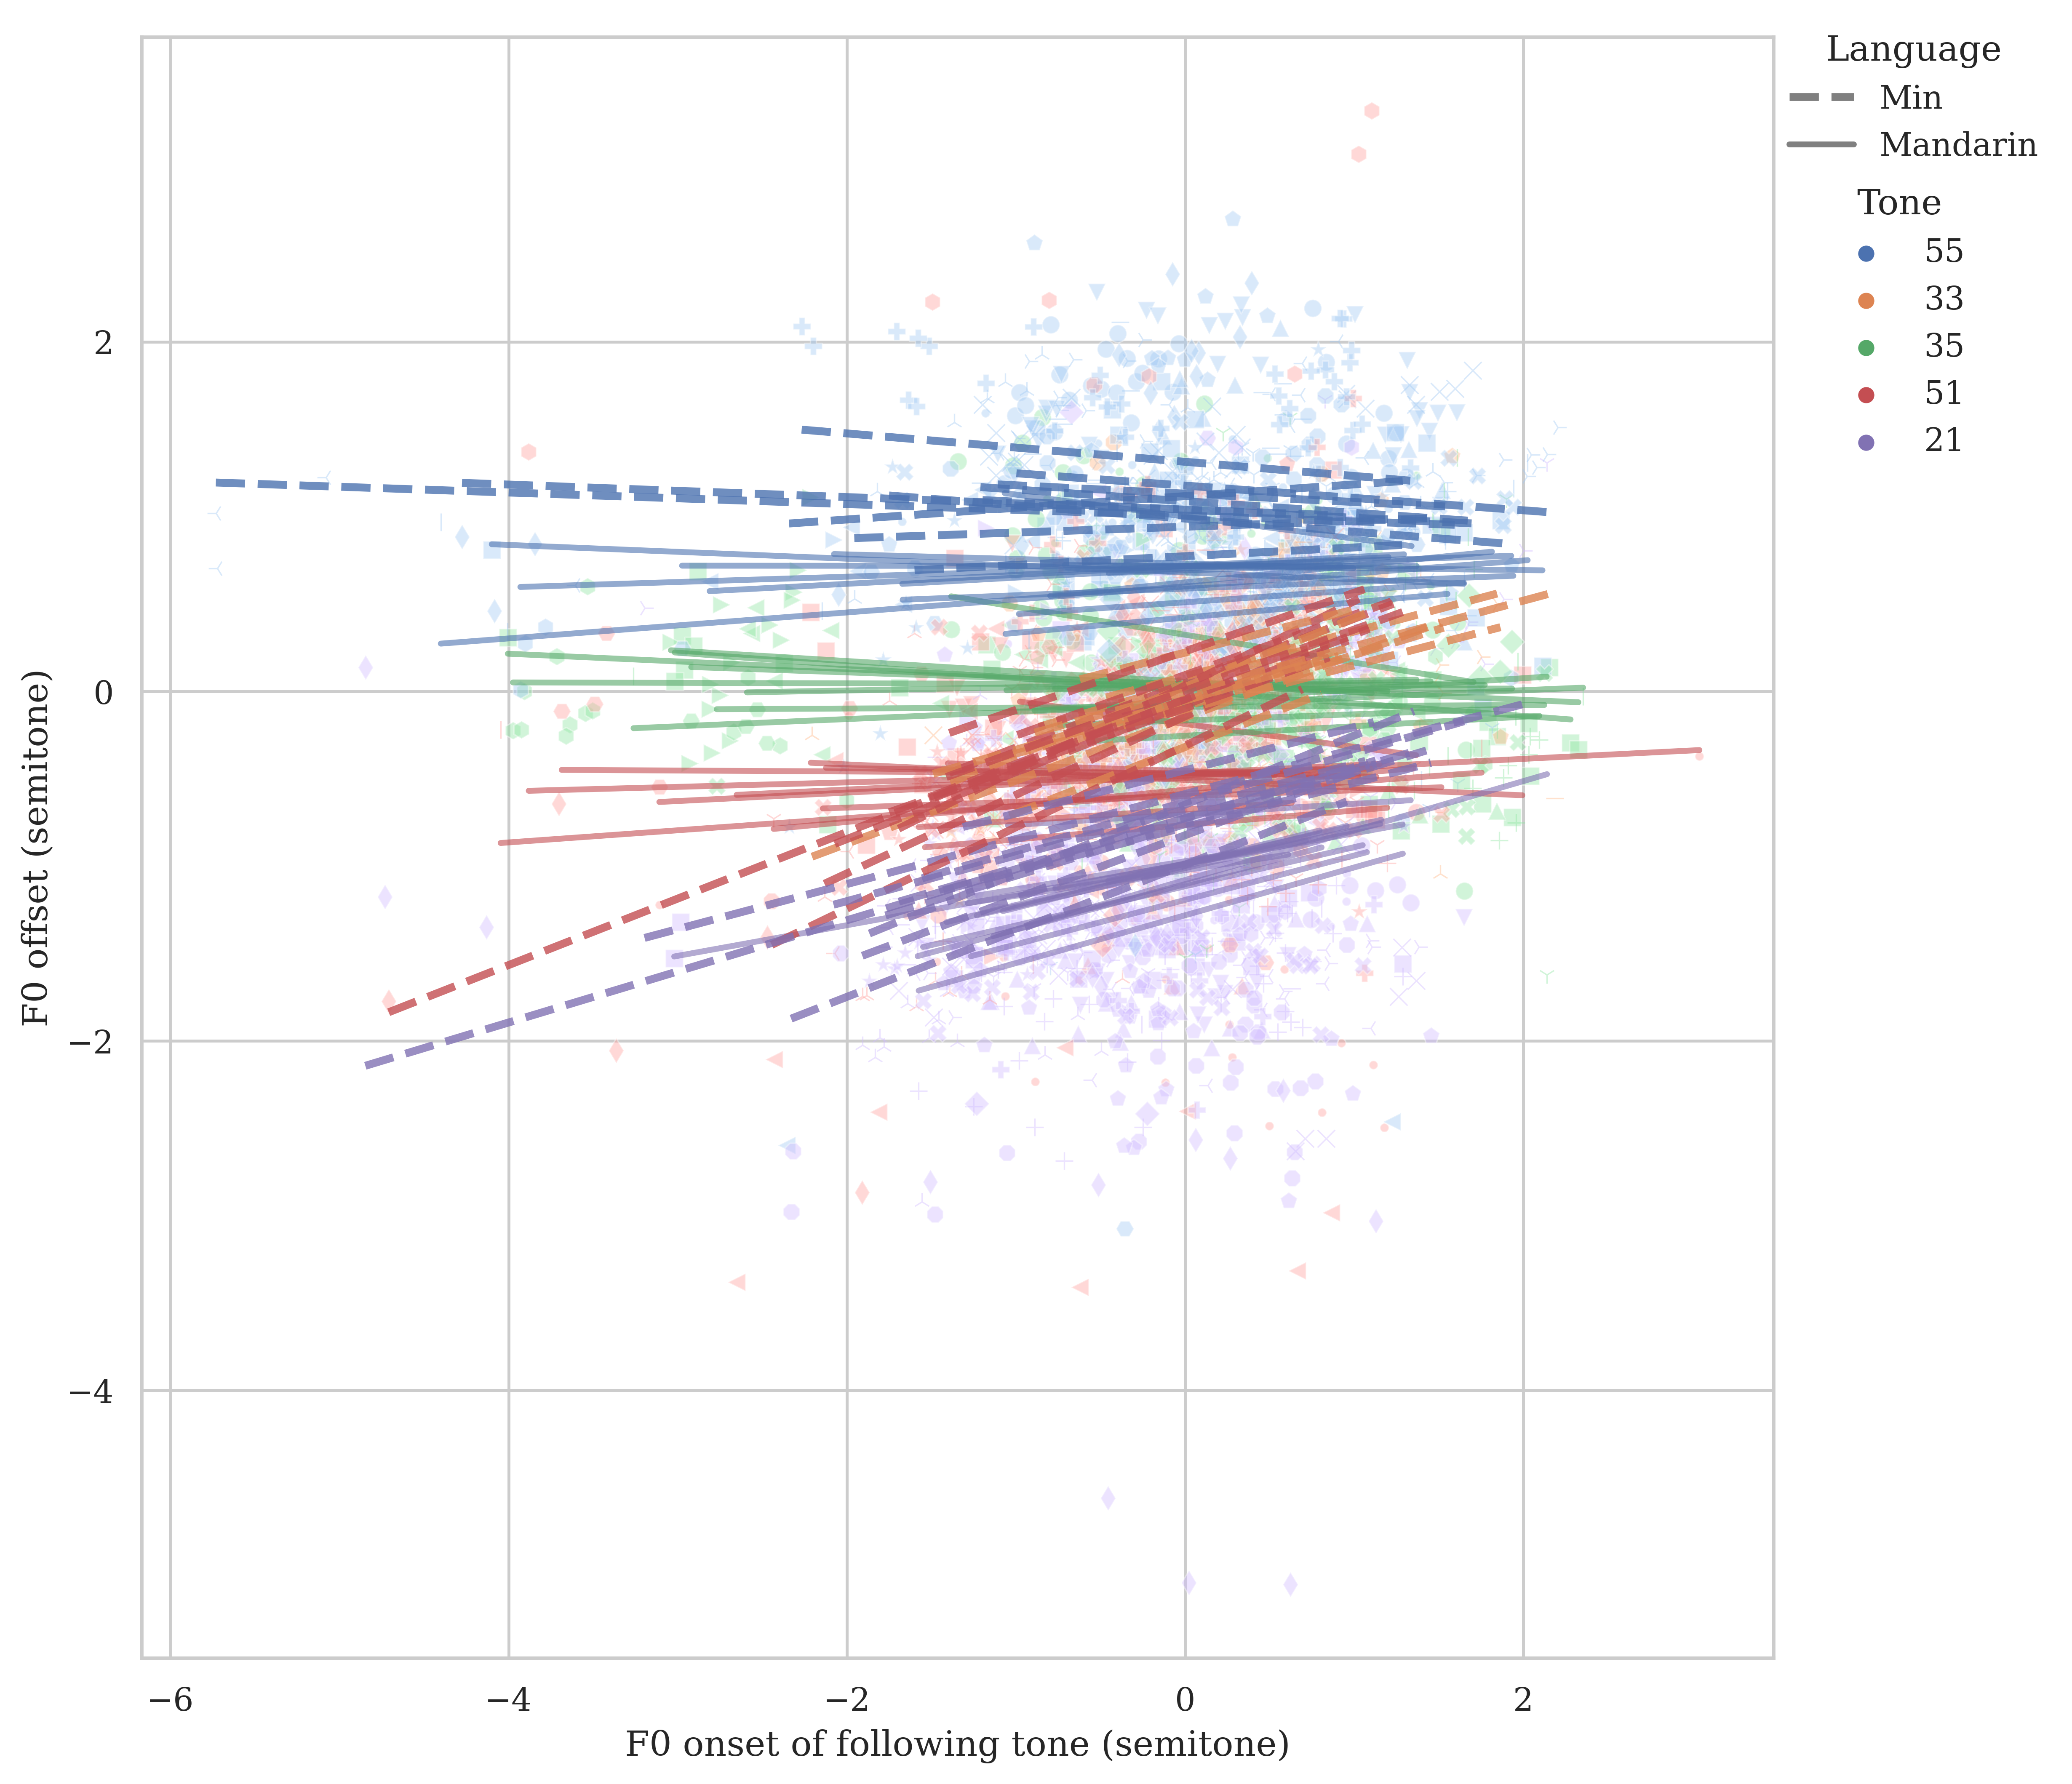
\includegraphics[scale=.45, trim={0 .5cm 0 0}]{figures/E1/Anticipatory.png}
%\caption{Fitted LMM model of tone onsets and offsets in anticipatory positions.}
%\label{Figure:LMMAnticipatory}
%\end{figure}

In general, tonal coarticulation in Taiwan Mandarin and Taiwan Southern Min were almost identical in both directionality and magnitudes. Symmetries were found in both languages, and no difference of magnitude was found. This can be summarized in tables \ref{table:MandarinMinDistribution} and \ref{table:MandarinMinDistributionComparison}.

\begin{flushleft}
\begin{table}[hbt!]
\begin{tabularx}{\textwidth}{l|X|X|}
\cline{2-3}
 & Magnitude & Direction \\
%\hhline{-::==}
\hhline{~|--}\noalign{\vspace*{\doublerulesep}}
\hhline{-||--}
\multicolumn{1}{|X||}{Carry-over} & \multirow{2}{*}{Equally strong} & \multirow{2}{*}{Assimilatory}\\
\hhline{|-||~~}
\multicolumn{1}{|X||}{Anticipatory} &  & \\
\hhline{|-||-|-|}
\end{tabularx}
\caption{Distribution of tonal coarticulation in Taiwan Mandarin and Taiwan Southern Min}
\label{table:MandarinMinDistribution}
\end{table}
\end{flushleft}

\begin{flushleft}
\begin{table}[hbt!]
\begin{tabularx}{\textwidth}{l|X|X|}
\cline{2-3}
 & Carry-over & Anticipatory \\
\hhline{~|--}\noalign{\vspace*{\doublerulesep}}
\hhline{-||--}
\multicolumn{1}{|X||}{Taiwan Mandarin} & \multirow{2}{*}{Equally strong} & \multirow{2}{*}{Equally strong}\\
\hhline{|-||~~}
\multicolumn{1}{|X||}{Taiwan Southern Min} &  & \\
\hhline{|-||-|-|}
\end{tabularx}
\caption{Comparison of tonal coarticulation between Taiwan Mandarin and Taiwan Southern Min}
\label{table:MandarinMinDistributionComparison}
\end{table}
\end{flushleft}

\section{Normalization for tonal coarticulation in Taiwan Mandarin and Taiwan Southern Min}
Fitted falling tone responses of the the monolingual and bilingual groups in Mandarin and Southern Min are shown in Figure \ref{Figure:E2Raw}.

\begin{figure}[hbt!]
\centering
\begin{subfigure}[b]{.45\textwidth}
\centering
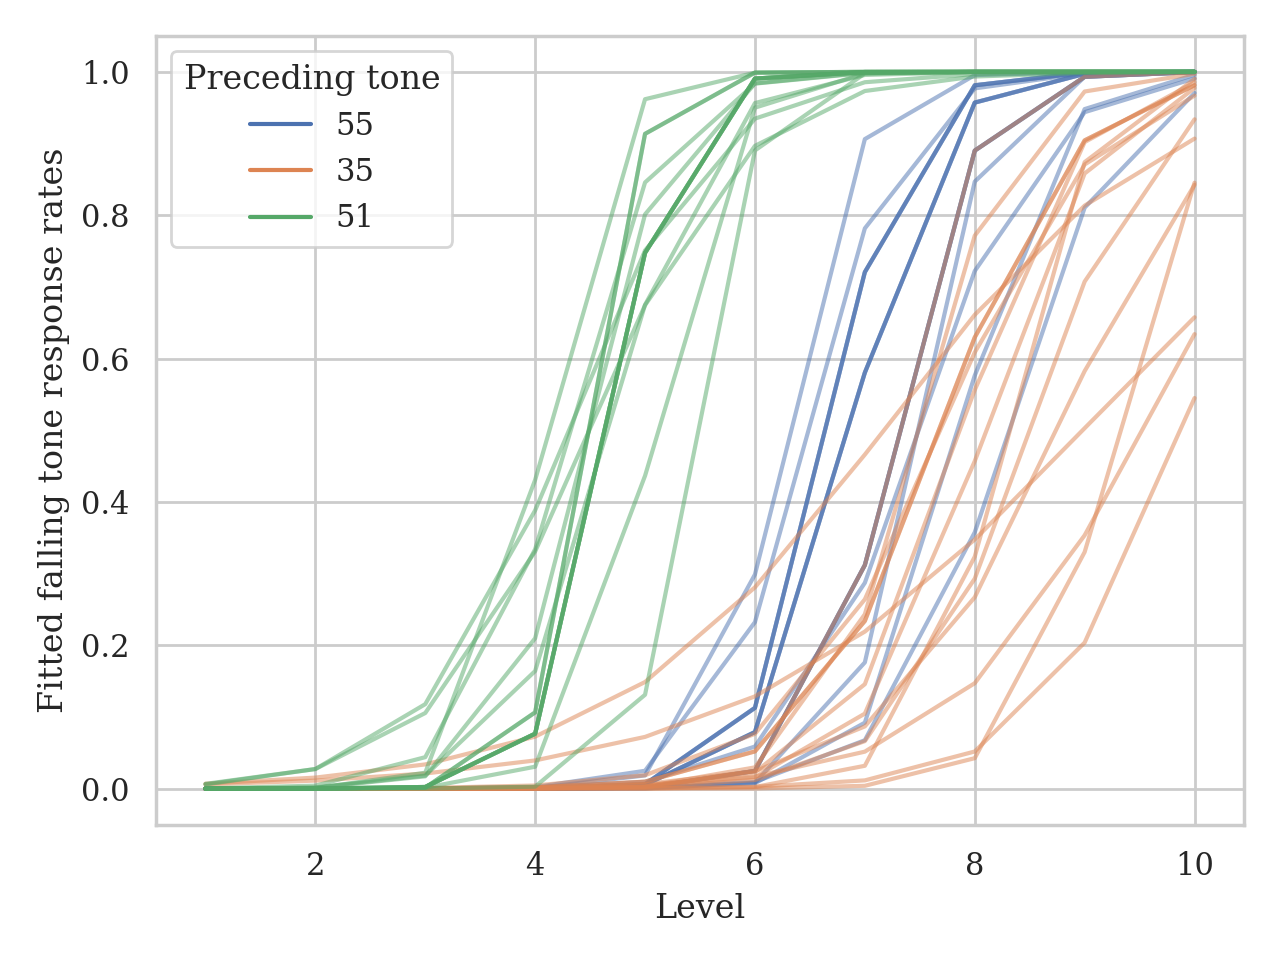
\includegraphics[width=\textwidth]{figures/E2/Mandarin_monolingual_E2_raw.png}
\end{subfigure}
\hfill
\begin{subfigure}[b]{.45\textwidth}
\centering
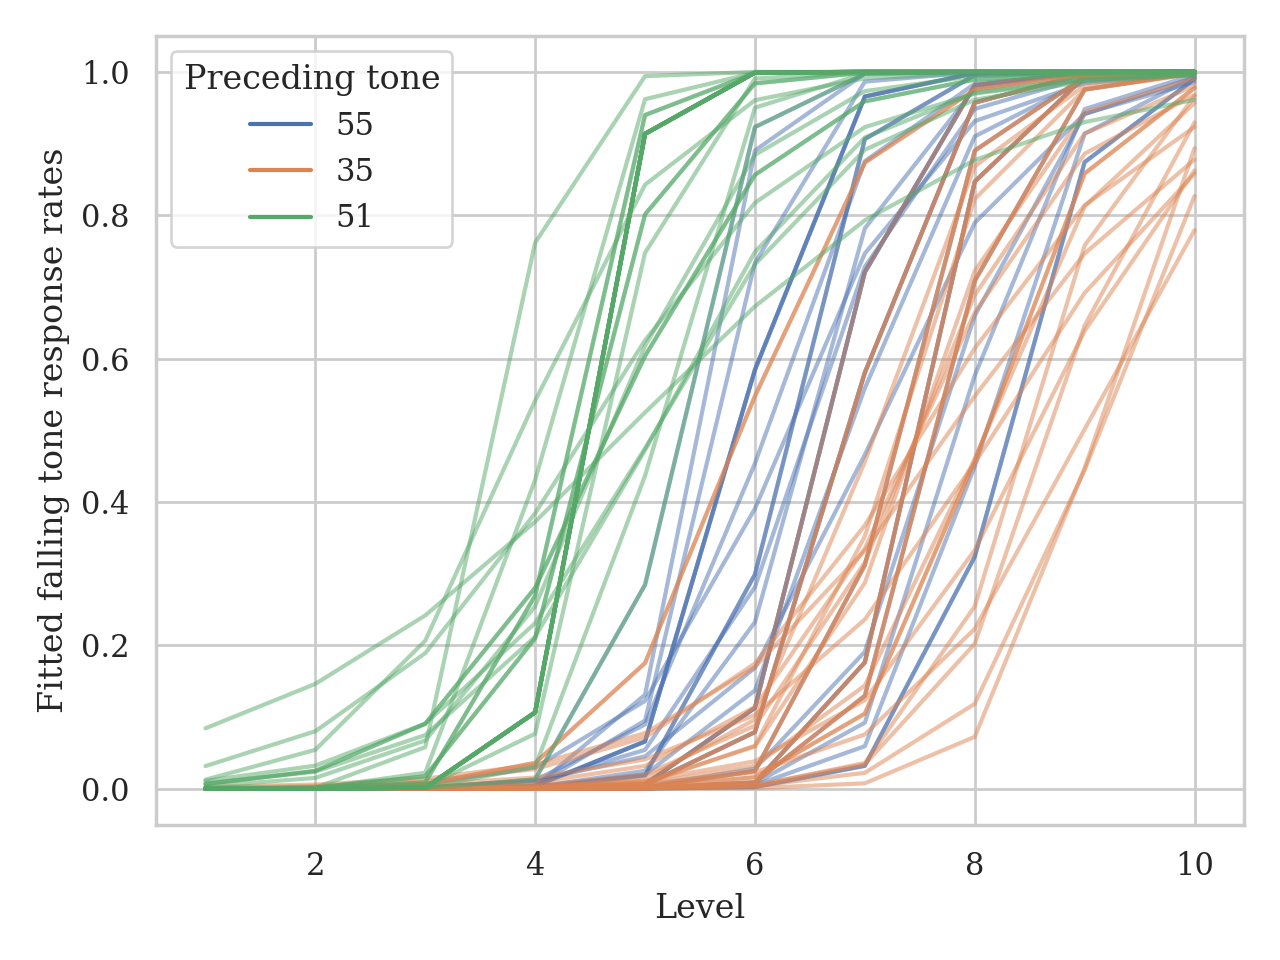
\includegraphics[width=\textwidth]{figures/E2/Mandarin_bilingual_E2_raw.png}
\end{subfigure}
\hfill
\begin{subfigure}[b]{.45\textwidth}
\centering
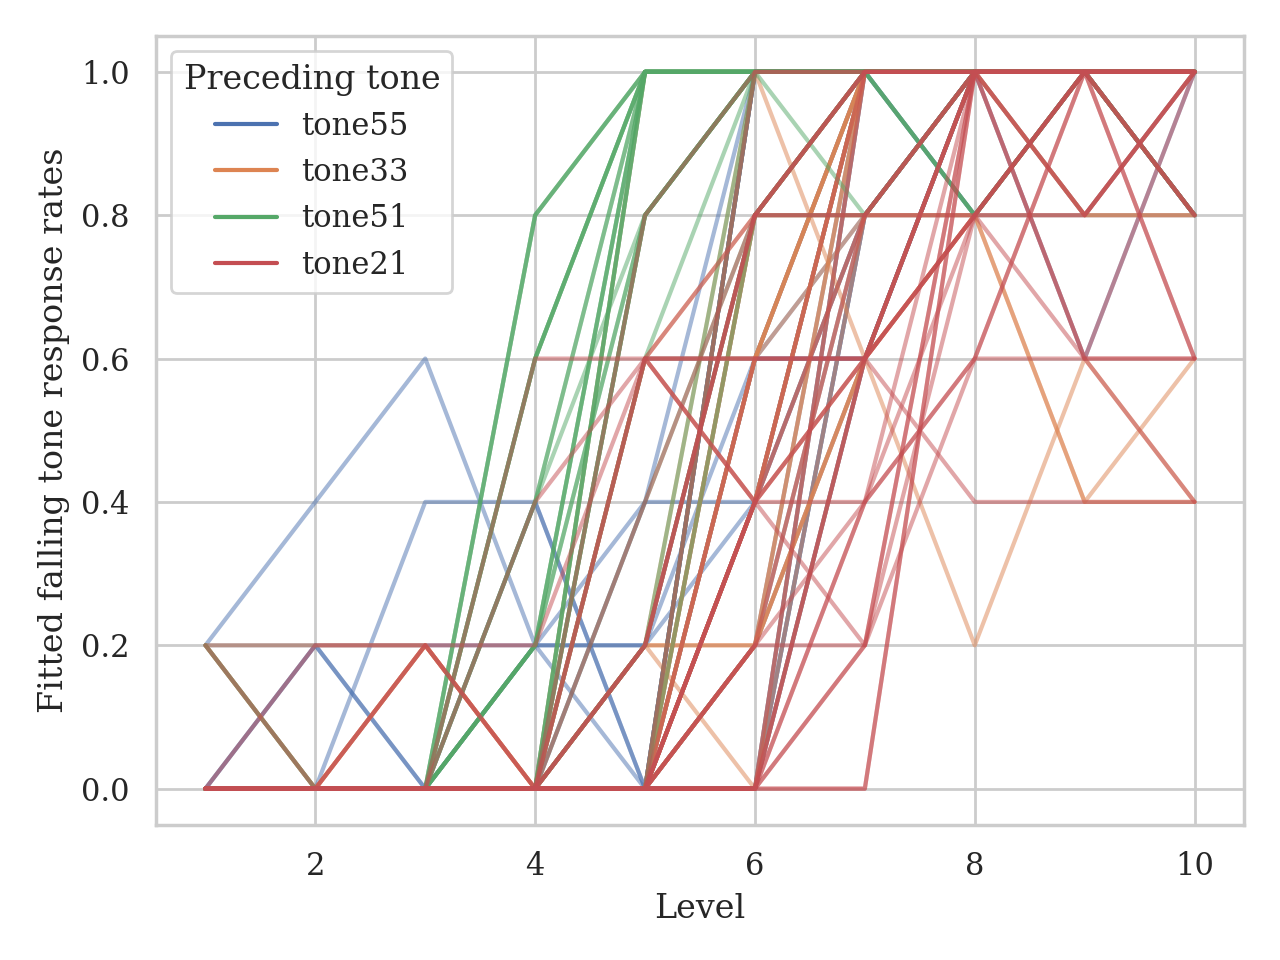
\includegraphics[width=\textwidth]{figures/E2/Min_E2_raw.png}
\end{subfigure}
\caption{Falling tone response percentages in Experiment 2 (top left: Mandarin (monolingual); top right: Mandarin (bilingual); bottom: Southern Min).}
\label{Figure:E2Raw}
\end{figure}

Upon first sight, we see an obvious difference between the monolingual group's Mandarin results and the bilingual group's Southern Min results, with the latter being generally narrower. The means of the maximum distances between these low-tone-to-falling-tone responses on the 0.25 and 0.75 thresholds are shown in Figure \ref{Figure:DistBoxPlot}.

\begin{figure}[hbt!]
\centering
\begin{subfigure}[b]{.49\textwidth}
\centering
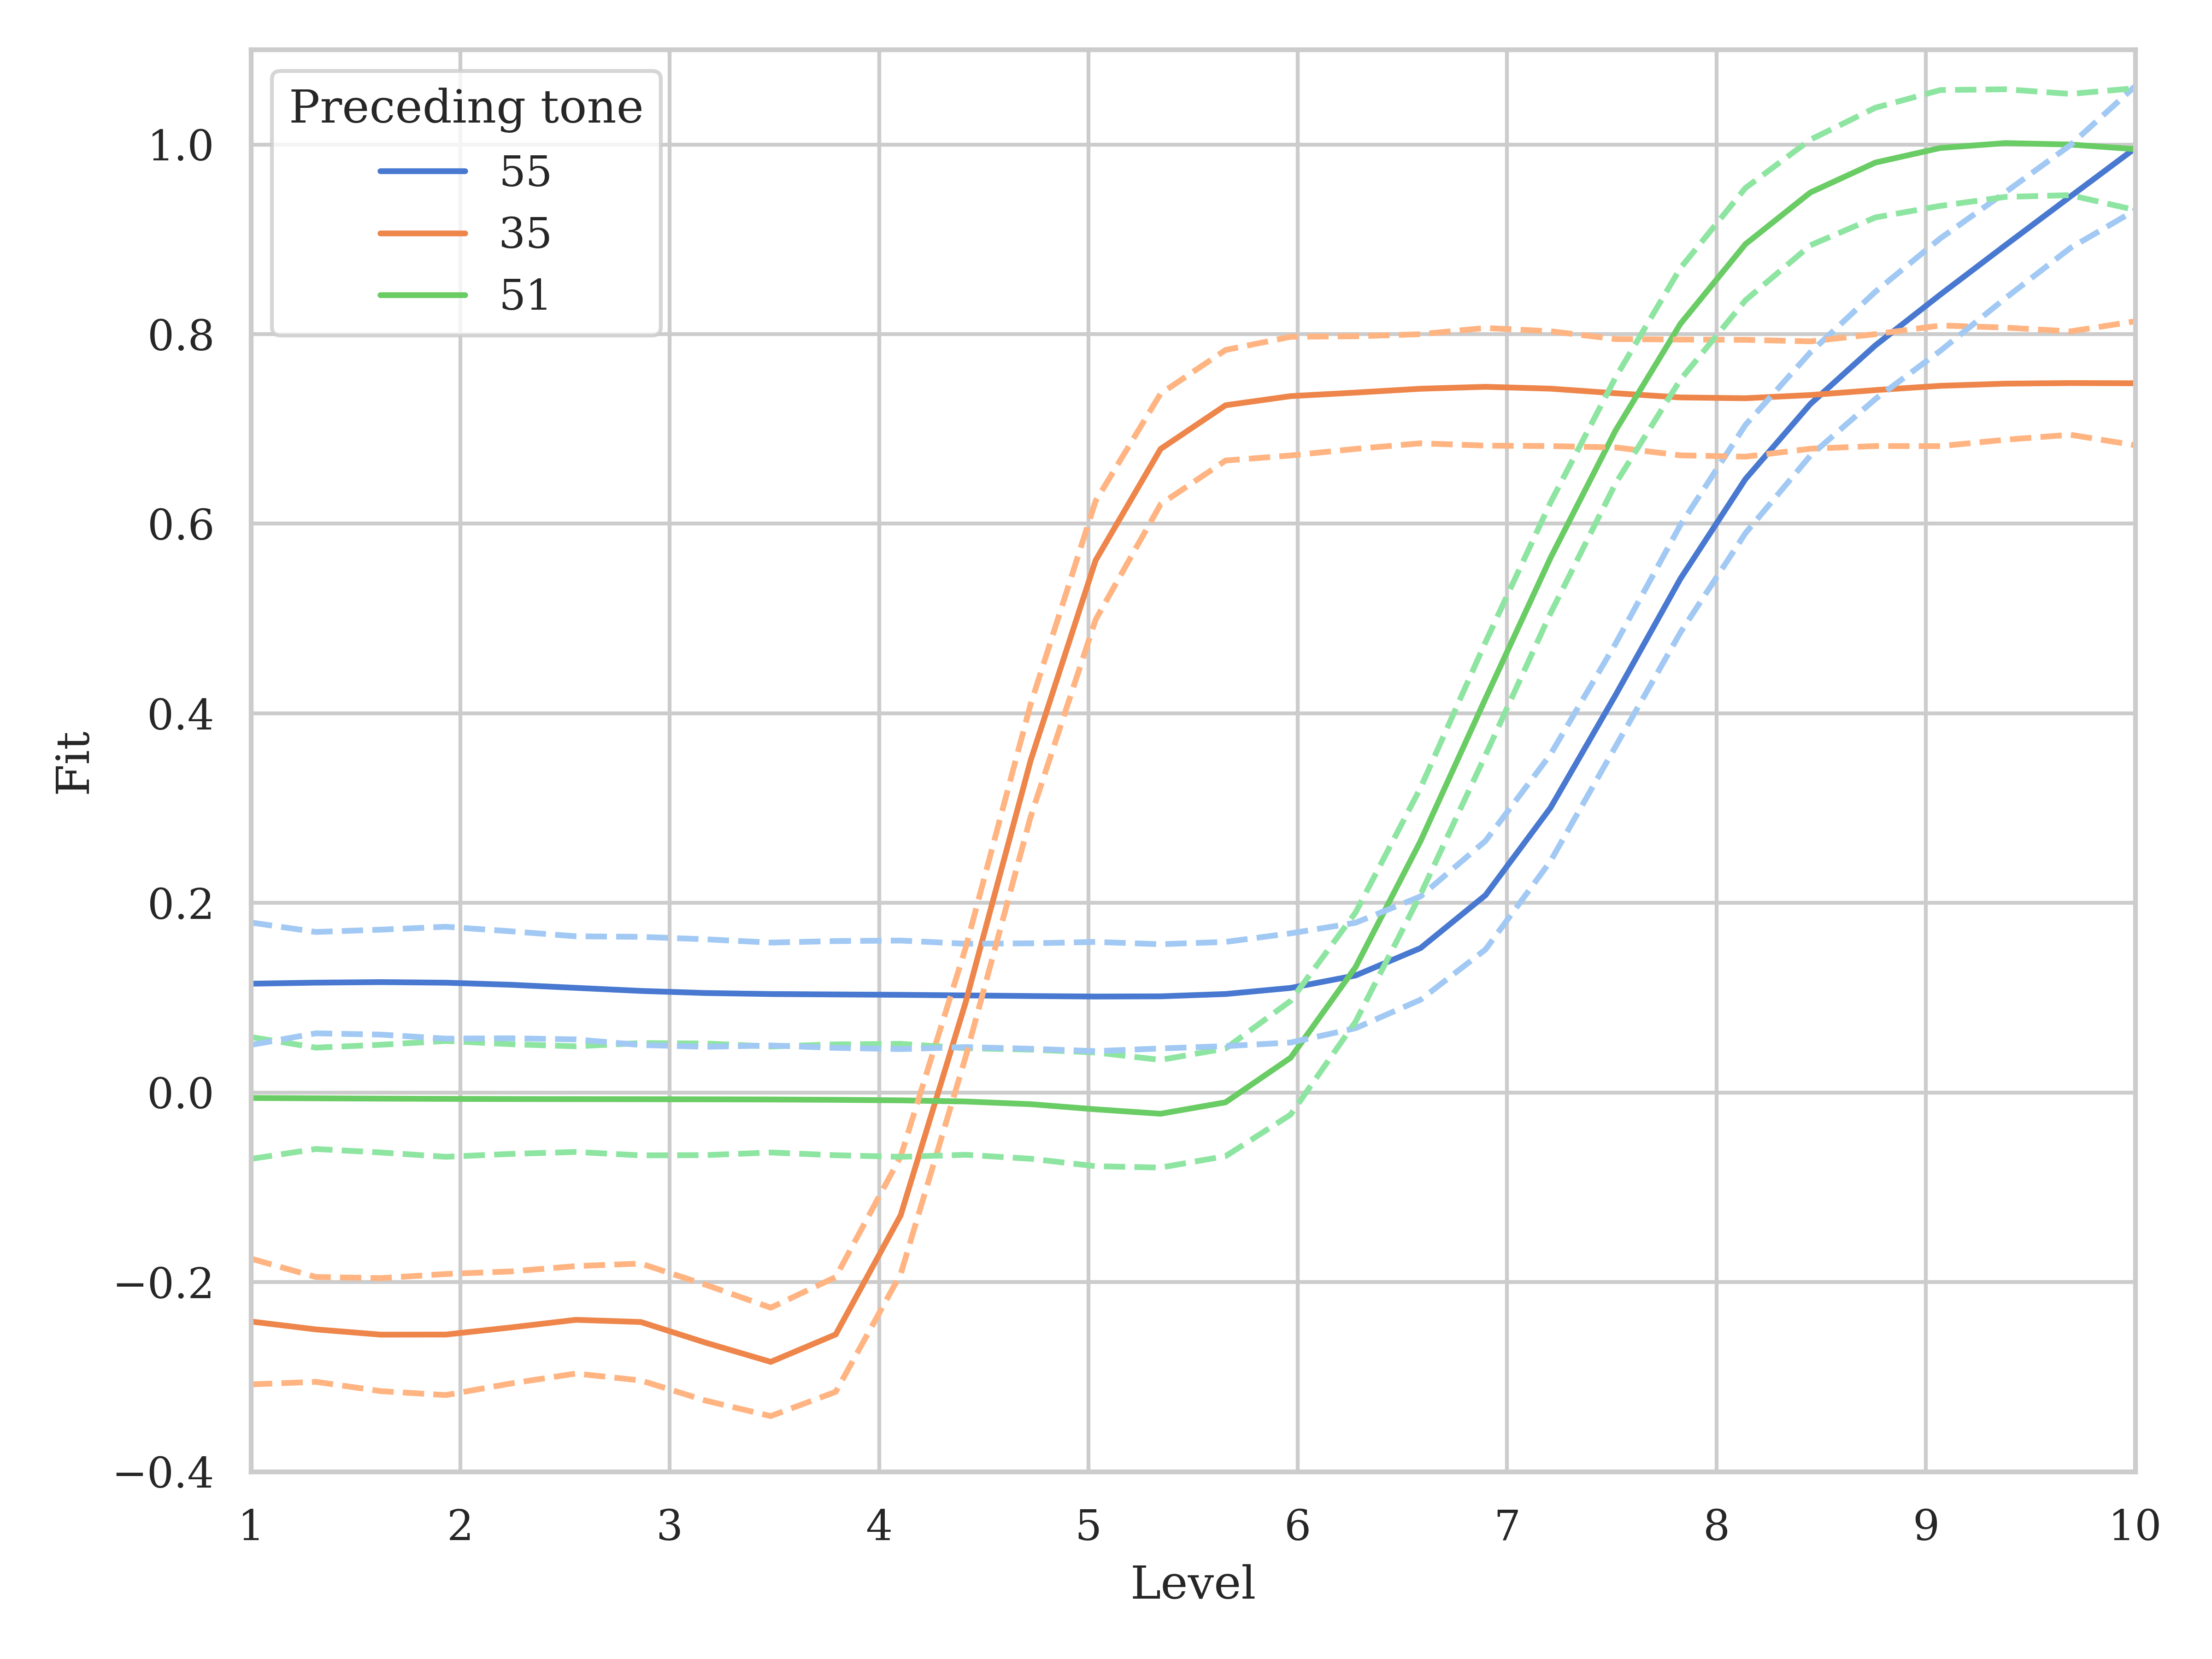
\includegraphics[width=\textwidth]{figures/E2/Mandarin_GAMM.png}
\end{subfigure}
\hfill
\begin{subfigure}[b]{.49\textwidth}
\centering
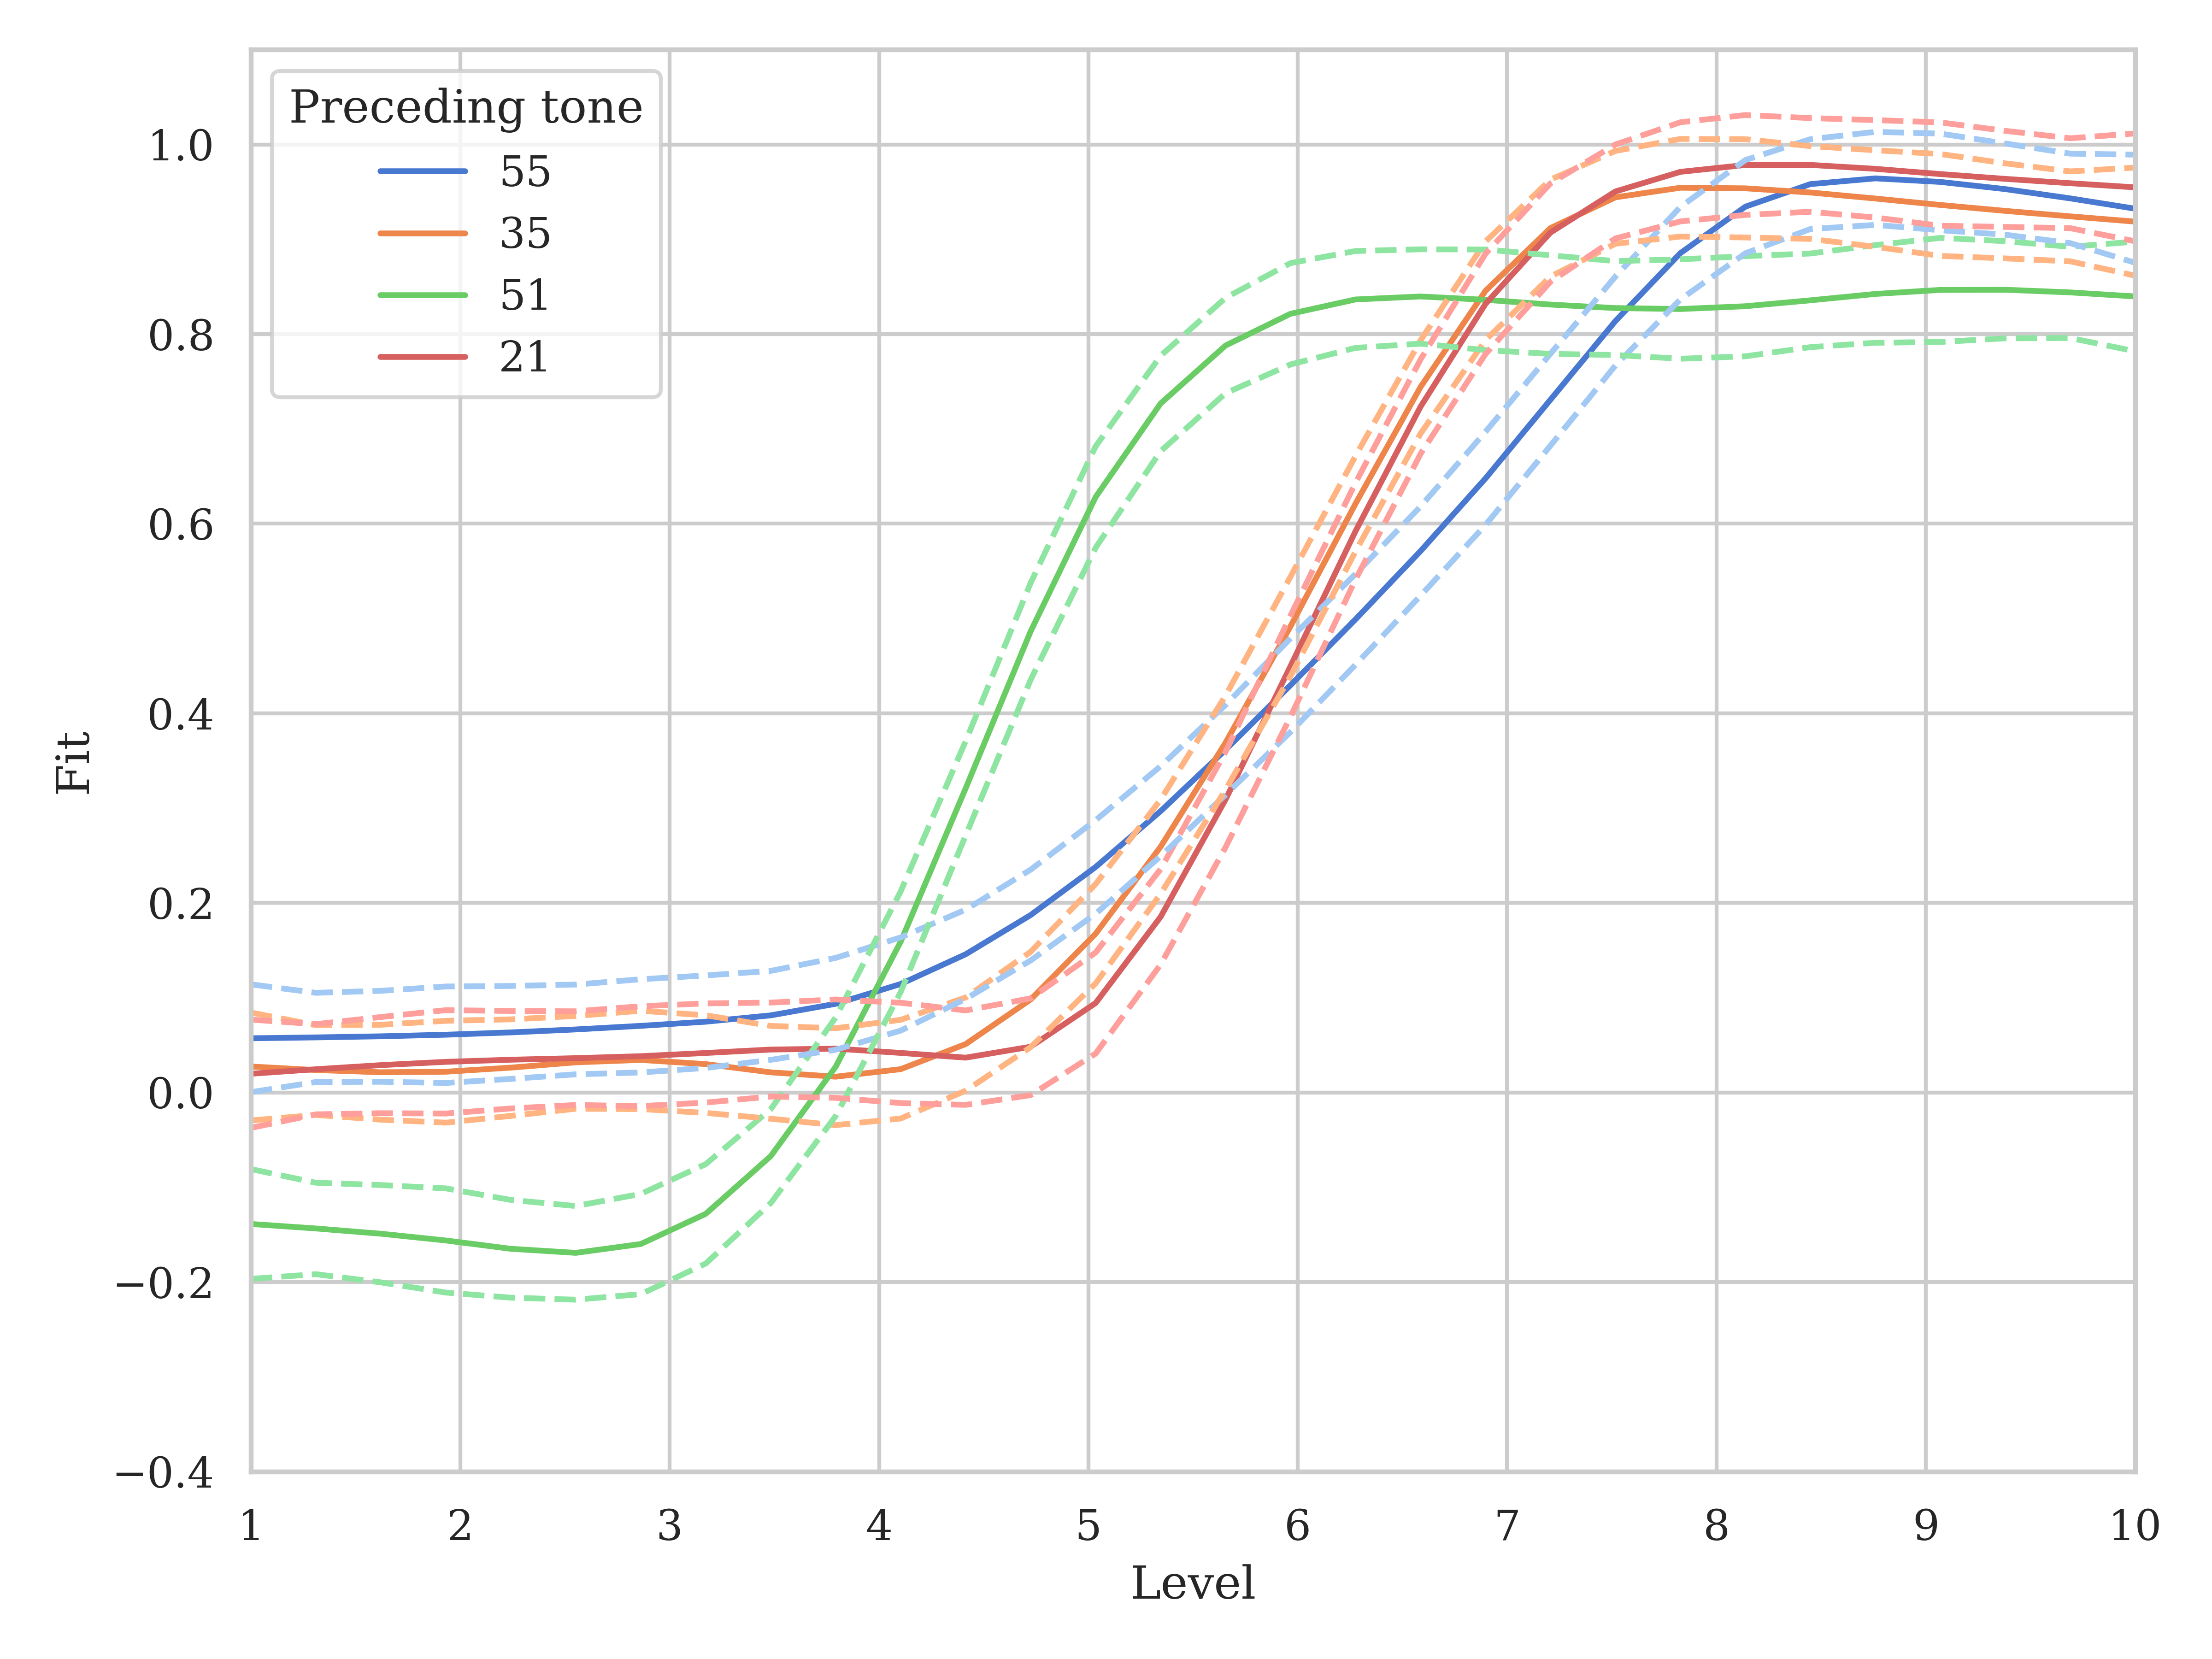
\includegraphics[width=\textwidth]{figures/E2/Min_GAMM.png}
\end{subfigure}
\caption{Fitted splines in Experiment 2.}
\label{Figure:DistBoxPlot}
\end{figure}

%A one-way ANOVA revealed that there was significant difference between at least two of the Southern Min results, and the monolingual and bilingual groups' Mandarin results (F(2, 62)=5.53, p<.01**).

As mentioned in Section \ref{section:Experiment2}, this measurement serves as a means of quantification of the magnitudes of perceptual normalization for tonal coarticulation. A simple t-test showed that the the distances in Taiwan Southern Min are significantly shorter than the distances in Mandarin on the monolingual group (p<.001**)\footnote{Post-hoc power analyses have been done for this and following reported significant results, all results gained a power of 71\% or higher.}. This suggests that normalization for tonal coarticulation was of a smaller amplitude in Taiwan Southern Min than in Taiwan Mandarin. Interestingly, this difference between Mandarin and Southern Min was present not only between groups, but also within subjects, as shown in Figure \ref{Figure:DistBilingualBoxPlot}. A paired t-test showed that even on the same speakers of the advanced bilingual group, this normalization was stronger in Mandarin than in Southern Min (p<.05*). This linguistic discrepancy, however, faded away on intermediate bilinguals (p=.32).

\begin{figure}[hbt!]
\centering
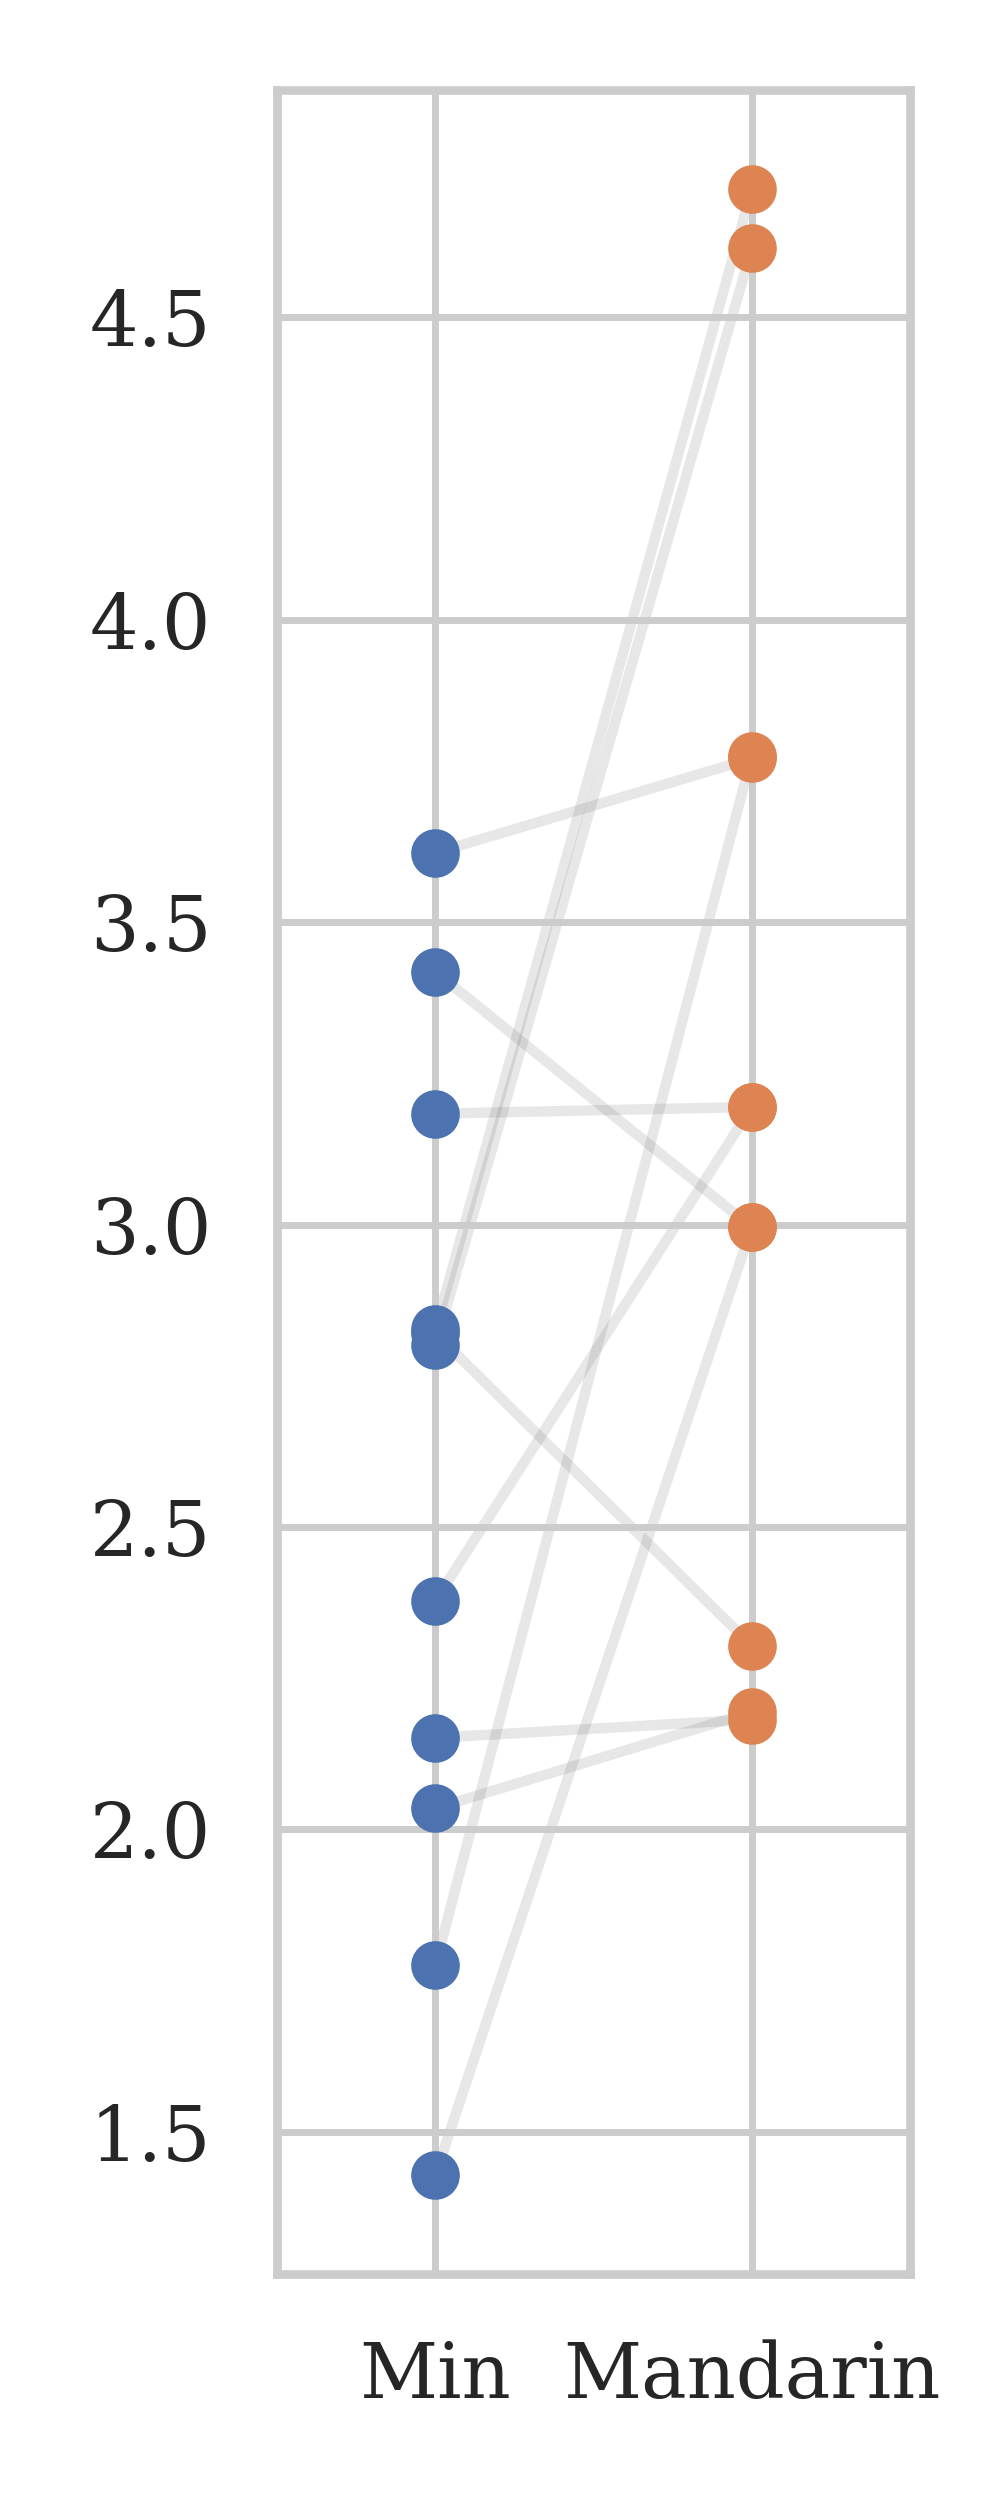
\includegraphics[width=.3\textwidth, trim={0 .5cm 0 0}]{figures/E2/Result_bilingual.png}
\caption{Pairwise comparison of calculated mean maximum distances (level) of advanced bilingual subjects in Experiment 2.}
\label{Figure:DistBilingualBoxPlot}
\end{figure}

\section{Tone boundaries between the low tone and the falling tone in Mandarin and Taiwan Southern Min}

Fitted acceptance rates of the falling tone and the low tone in Mandarin and Southern Min of the monolingual and bilingual groups are shown in Figure \ref{Figure:E3Raw}.

\begin{figure}[hbt!]
\centering
\begin{subfigure}[b]{.45\textwidth}
\centering
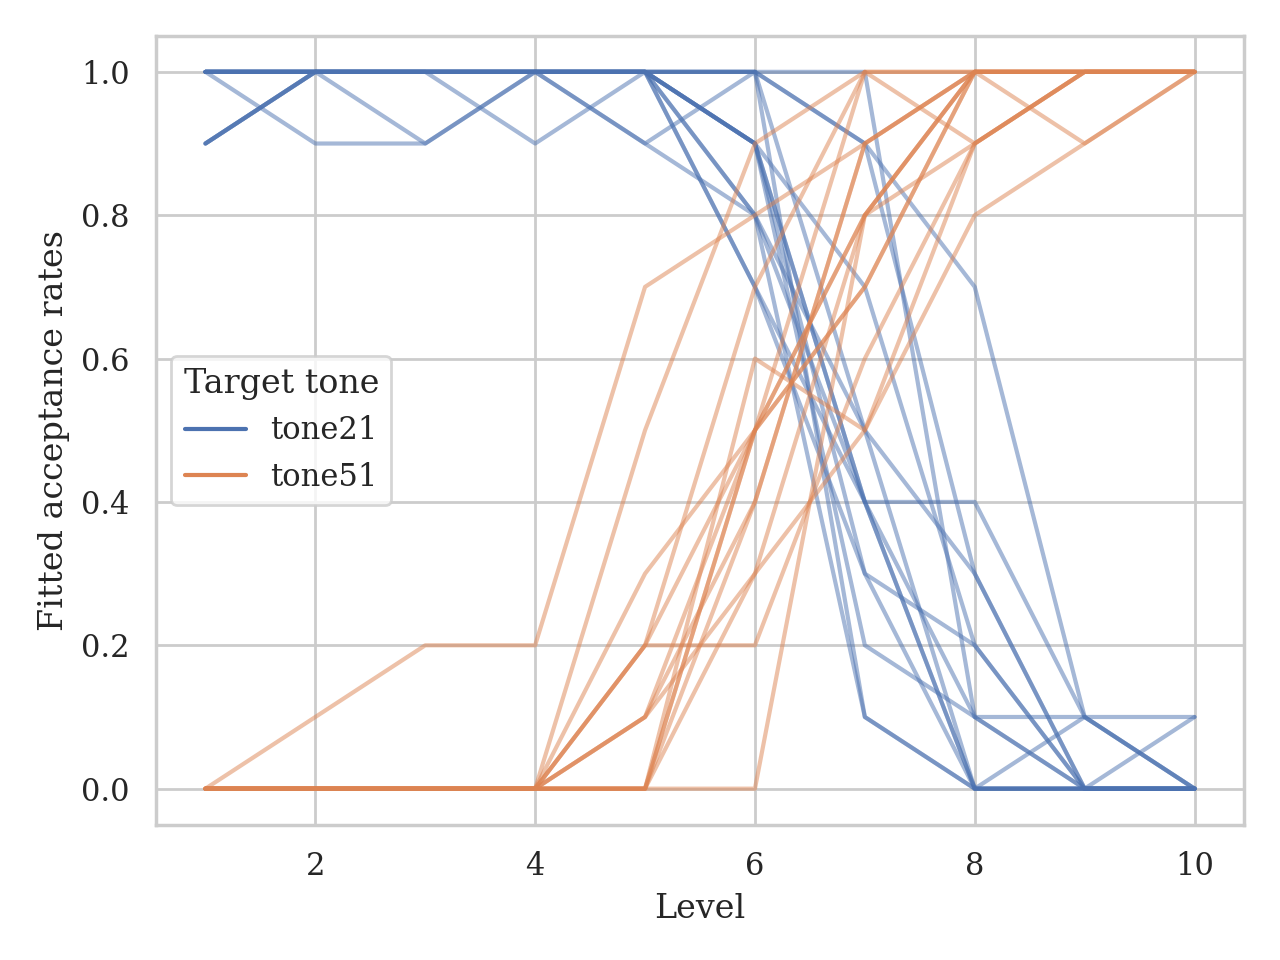
\includegraphics[width=\textwidth]{figures/E3/Mandarin_monolingual_E3_raw.png}
\end{subfigure}
\hfill
\begin{subfigure}[b]{.45\textwidth}
\centering
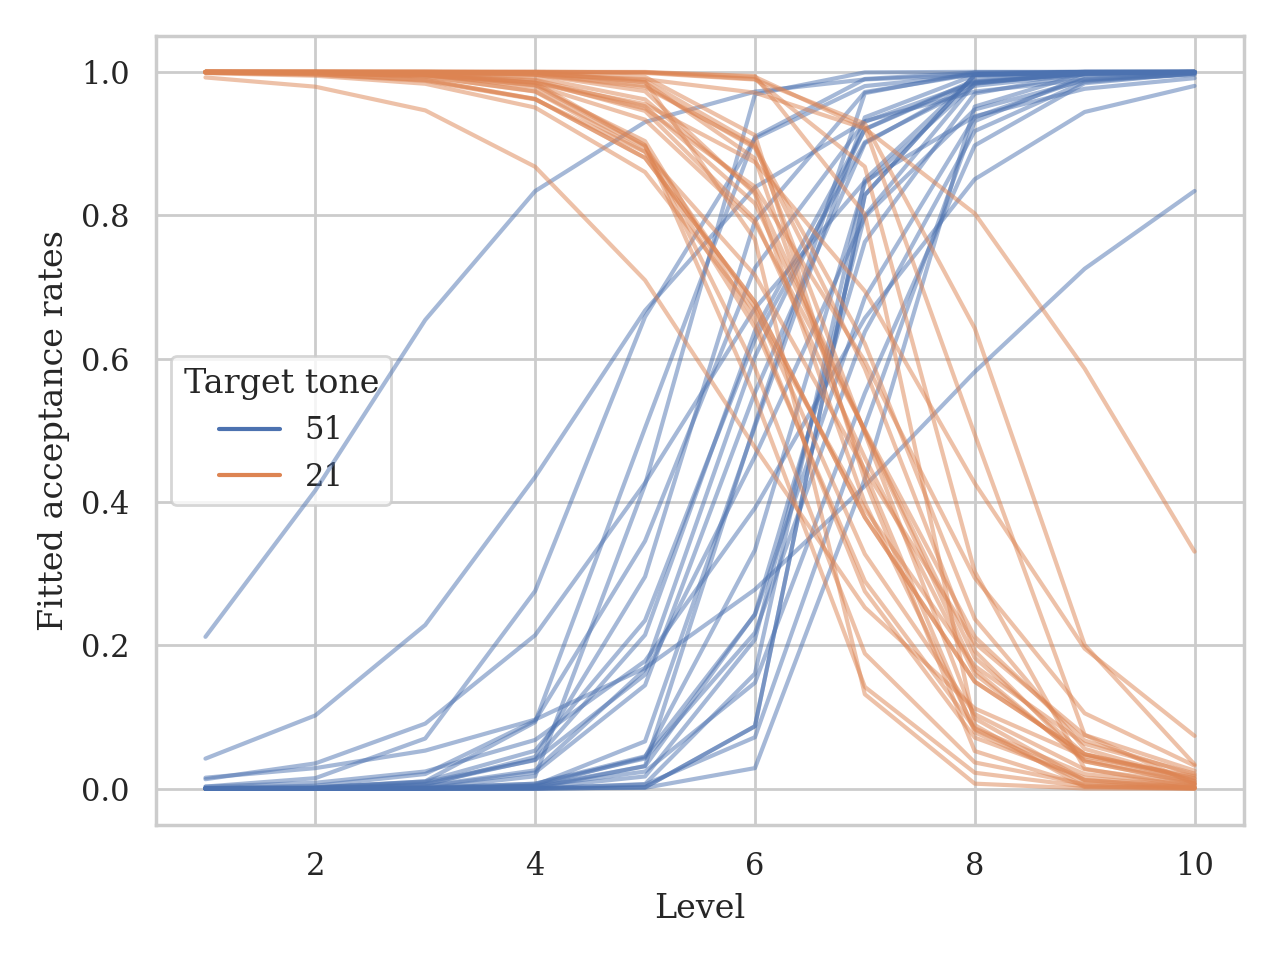
\includegraphics[width=\textwidth]{figures/E3/Mandarin_bilingual_E3_raw.png}
\end{subfigure}
\hfill
\begin{subfigure}[b]{.45\textwidth}
\centering
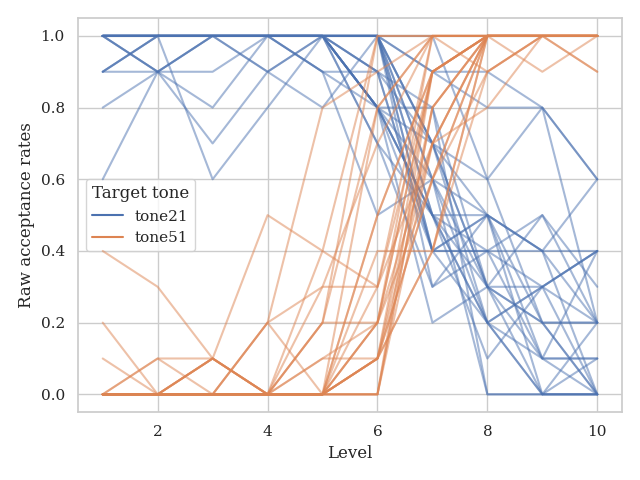
\includegraphics[width=\textwidth]{figures/E3/Min_E3_raw.png}
\end{subfigure}
\caption{Acceptance rates in Experiment 3 (top left: Mandarin (monolingual); top right: Mandarin (bilingual); bottom: Southern Min).}
\label{Figure:E3Raw}
\end{figure}

In general, we see that the falling tone had stricter boundaries than the low tone. Maximum slopes of the regressions of the two tones in Mandarin and Southern Min are shown in Figure \ref{Figure:E3BoxPlot}.

\begin{figure}[hbt!]
\centering
\begin{subfigure}[b]{.45\textwidth}
\centering
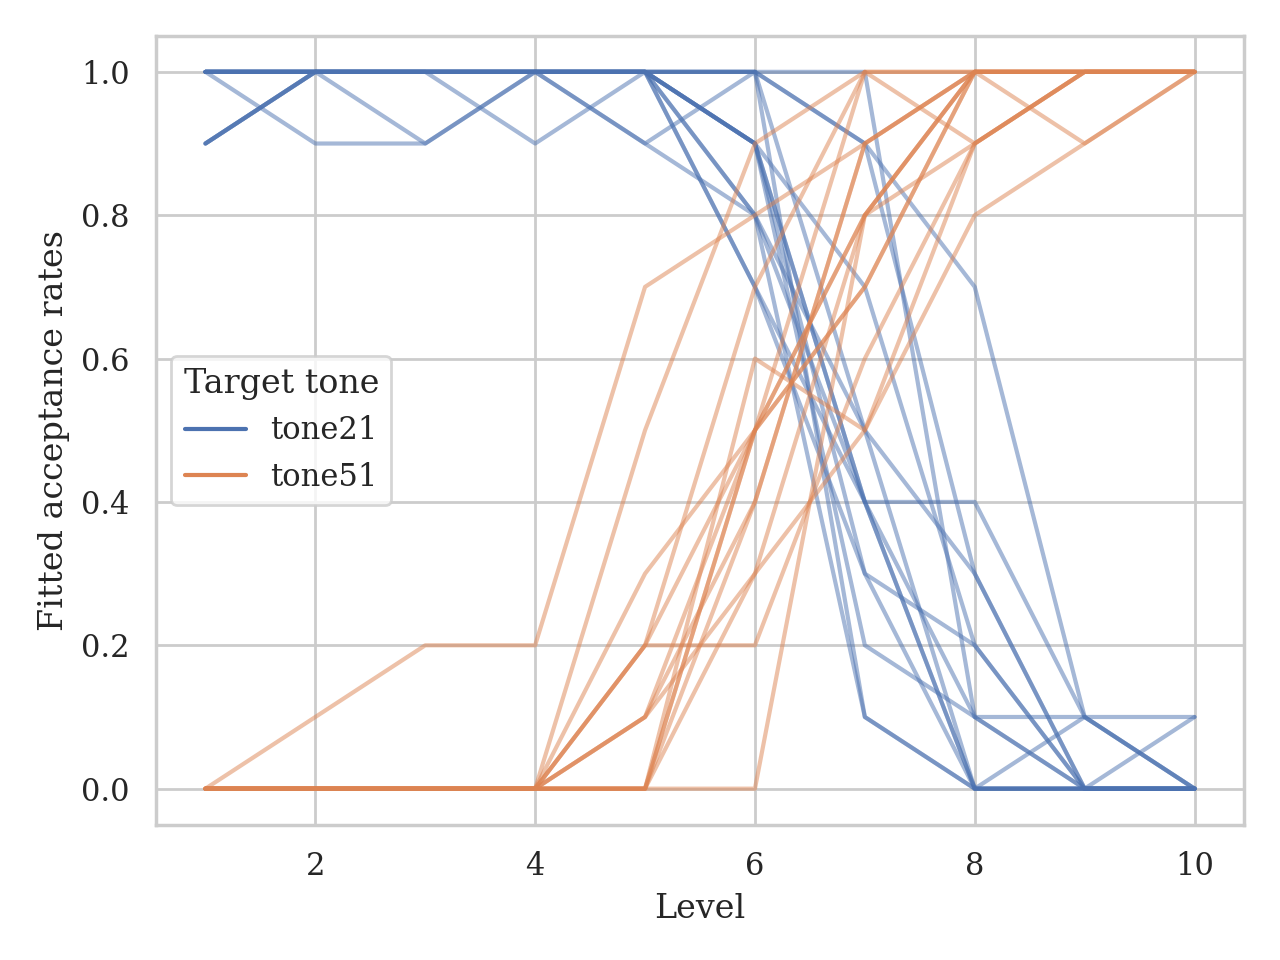
\includegraphics[width=\textwidth]{figures/E3/Mandarin_monolingual_E3_raw.png}
\end{subfigure}
\hfill
\begin{subfigure}[b]{.45\textwidth}
\centering
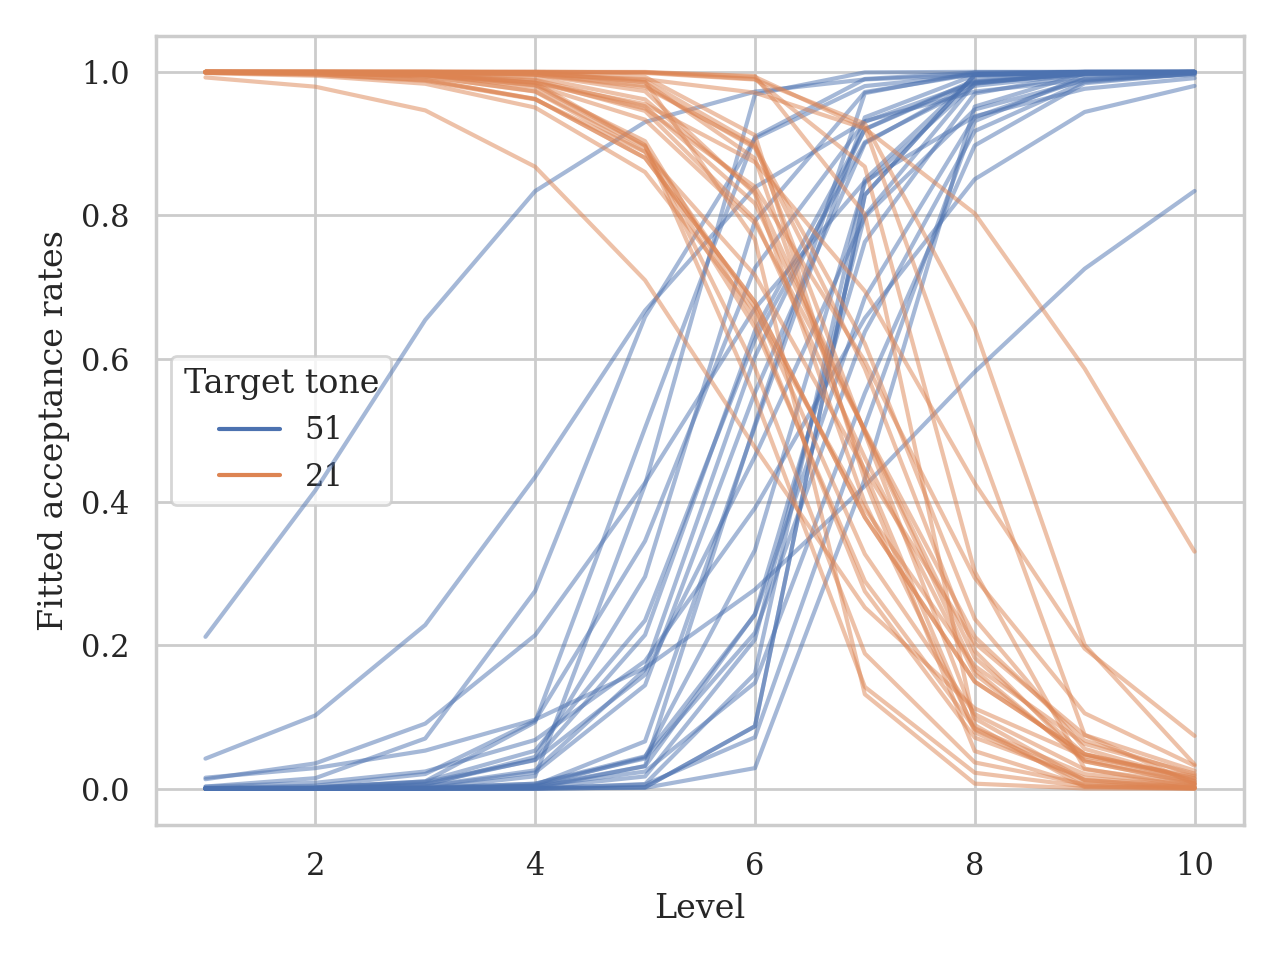
\includegraphics[width=\textwidth]{figures/E3/Mandarin_bilingual_E3_raw.png}
\end{subfigure}
\hfill
\begin{subfigure}[b]{.45\textwidth}
\centering
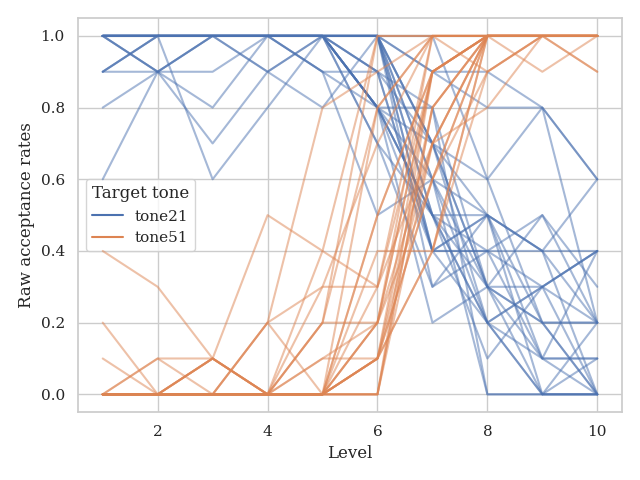
\includegraphics[width=\textwidth]{figures/E3/Min_E3_raw.png}
\end{subfigure}
\caption{Acceptance rates in Experiment 3 (top left: Mandarin (monolingual); top right: Mandarin (bilingual); bottom: Southern Min).}
\label{Figure:E3Raw}
\end{figure}

%Two one-way ANOVA's were done to examine the differences among the the maximum slopes of the bilingual group's Southern Min and Mandarin regression lines, and the monolingual group's Mandarin regression lines for falling and low tones respectively. For falling tone regression maximum slopes, no significant difference was found (F(2, 62)=.65, p=.52). For low tone regression maximum slopes, at least one of the three language$\times$group combinations were found to be different (F(2, 62)=13.23, p<.001***). A Simple t-test showed that bilingual subjects' Min low tone regression maximum slopes were significantly smaller than monolingual subjects' Mandarin results (p<.001***). A paired t-test revealed such linguistic difference was kept even within the bilingual subjects (p<.05*).
%
%To further investigate whether differences would be found when bilingual subjects were advanced speakers only, other two one-way ANOVA's were done again with the intermediate bilingual group's data taken out. This time, falling tone results were found to be significantly different between at least one of the language$\times$group combinations (F(2, 62)=5.31, p<.05*), and so were the low tone results (F(2, 62)=6.76, p<.01**).

Simple t-tests were done to investigate the differences between the bilingual group's Southern Min results and the monolingual speakers' Mandarin results for the falling tones and low tones, respectively. No significant differences were found between the maximum slopes of bilinguals' Southern Min falling tone and those of their Mandarin counterparts' Mandarin falling tone (p=.33). However, for the low tones, the monolingual group's Mandarin slopes were significantly steeper than the bilingual group's Southern Min slopes (p<.001***).

To further investigate whether differences would be found when the bilingual subjects were advanced speakers only. Simple t-tests were also done with exclusion of the intermediate bilingual group's data. It was revealed that the slope distributions were opposite between monolingual speakers' Mandarin and advanced bilingual speakers' Southern Min. Maximum slopes of the falling tone regressions were larger in the advanced bilingual speakers' Southern Min (p<.05*), while when it turned to the low tone's acceptance, it was the monolingual speaker's Mandarin that had steeper slopes (p<.01**). Recall that in Section \ref{section:Experiment3}, it is mentioned that the slopes are taken as indicators of the speakers' strictness on the tone boundaries. This suggests that when the monolingual speakers had stricter low tone boundaries in Mandarin, and that the advanced bilinguals had stricter falling tone boundaries in Southern Min. A paired t-test revealed that such linguistic difference was kept even within the bilingual subjects (both p's<.05*).

\section{Summary}
In this section, we have examined tonal coarticulation in Taiwan Mandarin and Taiwan Southern Min, and normalization and tone boundaries in the two languages. It is seen that while Taiwan Mandarin and Taiwan Southern Min exhibited rather similar distribution in terms of tonal coarticulation, Taiwan Southern Min was shown to be less influenced by the normalization effect of tonal coarticulation. Tone boundaries of the falling tone and the low tone in these two languages were also shown to be different. In the next chapter, we will discuss the significances of these discrepancies and of other results that we have seen in this section.